\documentclass[a4paper, 12pt]{article}

%  PREAMBULĖ
% ------------------------------------------------------------------------------

\usepackage[utf8]{inputenc}            % naudojama, kai .tex failas UTF-8 koduotės
\usepackage[T1]{fontenc}
\usepackage[L7x]{fontenc}              % nurodoma lietuviško teksto koduotė Latin-7
\usepackage[english]{babel}
\usepackage{microtype}                 % optimizuojami atstumai tarp raidžių žodyje
\usepackage{indentfirst}               % atitraukiama pirmoji naujo skyriaus eilutė
\setlength{\parindent}{1.27cm}
\setlength{\parskip}{0pt}
\usepackage{icomma}                    % po kablelio skaičiaus viduryje nebus tarpo
\usepackage{amsmath, amssymb}  % matematiniai simboliai ir konstrukcijos
\usepackage{fontspec}
\setmainfont{Times New Roman}
\usepackage{graphicx}                  % grafinių failų įterpimas ir kiti nustatymai
\usepackage{pdfpages}
\usepackage{booktabs}                  % reikalingas tvarkingoms lentelėms sudaryti
\usepackage{caption}                   % paveiksliukų ir lentelių užrašų formavimas
\usepackage{geometry}                  % paraščių ir kitų lapo parametrų nustatymai
\usepackage{hyperref}                  % interaktyvioms nuorodoms dokumente sukurti
\usepackage{ragged2e}
\usepackage{tabularx}
\usepackage{amsfonts}
\usepackage{blindtext}
\usepackage[
    backend=biber,
    style=apa,
    sortcites=true,
    sorting=nyt,
    maxcitenames=3,
    mincitenames=1
]{biblatex}
\DeclareLanguageMapping{english}{english-apa}
\addbibresource{source.bib}
\usepackage[acronym]{glossaries}
\usepackage{longtable}
\usepackage{subcaption}
\usepackage{tikz}
\usepackage{float}
\usepackage[toc,page,title]{appendix}
\usetikzlibrary{positioning}
\usepackage{tocloft}
\newlistof{loa}{exp}{List of Appendices}
\newcommand{\appendixtitle}[2]{
  \refstepcounter{loa}
  \addcontentsline{exp}{loa}{\protect\numberline{\theloa}#1}
  \noindent\textbf{#2}
  \vspace{0.5em}
}
\makeatletter
\renewcommand{\listofloa}{
  \begingroup
  \let\clearpage\relax
  \section*{List of Appendices}
  \@starttoc{exp}
  \endgroup
}
\makeatother
\geometry{      left = 3.0cm,          % paketo geometry parametrų nustatymai
               right = 2.0cm, 
                 top = 2.0cm, 
              bottom = 2.0cm
}

\captionsetup{format = hang,           % paketo caption parametrų nustatymai
           labelfont = bf,
           labelsep = period,
           tablename = Table,
          figurename = Figure
}

\hypersetup{ unicode = true,           % paketo hyperref parametrų nustatymai
         linktocpage = false, 
          colorlinks = true, 
           linkcolor = black,
           citecolor = blue,
            pdftitle = {VGTU FMF MKDf bakalaurinio darbo šablonas},
           pdfauthor = {Mindaugas Kazlavickas}
}

% PAPILDOMI PAKETAI IR NUSTATYMAI ----------------------------------------------

\usepackage{titlesec}                  % leidžia keisti skyriaus pavadinimo stilių
\titlelabel{\thetitle.\quad}           % dedamas taškas po skyriaus numeriu tekste

\titleformat{\section}
  {\bfseries\Large}
  {\thesection.}
  {1em}
  {}

\titleformat{\subsection}
  {\bfseries\normalsize}
  {\thesubsection.}
  {1em}
  {}

\titleformat{\subsubsection}
  {\normalsize\itshape}
  {\thesubsubsection.}
  {1em}
  {}
\let\tocnumdot\numberline              % uždeda tašką po skyriaus numeriu turinyje
\def\numberline#1{\tocnumdot{#1.}}     

\usepackage{setspace}
\onehalfspacing

\graphicspath{{figures/}}              % nustatome kelią iki paveiksliukų katalogo 

% ------------------------------------------------------------------------------
%  SUTRUMPINIMAI
\newacronym{sdt}{SDT}{Self-Determination-Theory}
\newacronym{vr}{VR}{Virtual Reality}
\newacronym{mda}{MDA}{Mechanics, Dynamics and Aesthetics (Framework)}
\newacronym{lms}{LMS}{Learning Management System}
\newacronym{fbm}{FBM}{Fogg's Behaviour Model}
\newacronym{cta}{CTA}{Call-To-Action}
\newacronym{svg}{SVG}{Scalable Vector Graphics}
\newacronym{json}{JSON}{JavaScript Object Notation}
\newacronym{api}{API}{Application Programming Interface}
\makeglossaries

\newcommand{\progresscalc}[2]{%
  \begin{equation}
  \text{Progress} = \frac{#1}{#2} \times 100\%%
  \end{equation}
}
% ------------------------------------------------------------------------------
%  DOKUMENTO PRADŽIA
% ------------------------------------------------------------------------------
\begin{document}
% ------------------------------------------------------------------ VIRŠELIS --
\begin{titlepage}
\setcounter{page}{-2}
\centering
%

\includegraphics{vgtu_herbas}\\[0.5\baselineskip]
%
{\Large\scshape VILNIUS GEDIMINAS TECHNICAL UNIVERSITY}\\[0.15\baselineskip]
{\scshape FACULTY OF FUNDAMENTAL SCIENCES}\\[0.15\baselineskip]
{\scshape DEPARTMENT OF GRAPHICAL SYSTEMS}\\[1.0\baselineskip]
%
\vspace{\fill}
%
{Mindaugas Kazlavickas}\\[3.0\baselineskip]
\MakeUppercase{\Large\bfseries Design of educational website on learning recognition by open badges applying gamification principles}\\[1.0\baselineskip]
\MakeUppercase{\Large\bfseries Mokomojo tinklalapio apie mokymosi pripažinimą atviraisiais ženkliukais projektavimas taikant sužaidybinimo principus}\\[0.3\baselineskip]

{Bachelor's degree final work}

\vspace{\fill}

Multimedia and Computer Design study programme, state code 6121BX025

Informatics Engineering specialization

Informatics study field


\vspace{\fill}
%
Vilnius, \the\year
\end{titlepage}
\newpage
\begin{titlepage}
\setcounter{page}{-1}
\centering
%
{\Large\scshape VILNIUS GEDIMINAS TECHNICAL UNIVERSITY}\\[0.2\baselineskip]
{\scshape FACULTY OF FUNDAMENTAL SCIENCES}\\[0.2\baselineskip]
{\scshape DEPARTMENT OF GRAPHICAL SYSTEMS}\\[0.2\baselineskip]
%
\vspace{\fill}
%
%\begin{flushright}
%\parbox{6cm}{%
%APPROVED BY\\Head of Department
%\bigskip
%\begin{center}
%\hrule\medskip
%{\footnotesize (Signature)}\\[\baselineskip]
%\hrule\medskip
%{\footnotesize (Name, Surname)}\\[\baselineskip]
%\hrule\medskip
%{\footnotesize (Date)}
%\end{center}
%}
%\end{flushright}
%
\vspace{\fill}
%
{Mindaugas Kazlavickas}\\[3.0\baselineskip]

\MakeUppercase{\Large\bfseries Design of educational website on learning recognition by open badges applying gamification principles}\\[1.0\baselineskip]
\MakeUppercase{\Large\bfseries Mokomojo tinklalapio apie mokymosi pripažinimą atviraisiais ženkliukais projektavimas taikant sužaidybinimo principus}\\[1\baselineskip]

{Bachelor's degree final work}

\vspace{\fill}

Multimedia and Computer Design study programme, state code 6121BX025

Informatics Engineering specialisation

Informatics study field

\vspace{\fill}
%
\begin{flushright}
\parbox{0.7\textwidth}{
    \makebox[3cm][l]{\textbf{Supervisor:}}%
    \makebox[\dimexpr0.7\textwidth-3cm\relax][l]{\hrulefill}\\
    \hspace*{3cm}\makebox[\dimexpr0.7\textwidth-3cm\relax][c]{\scriptsize (Title, Name, Surname)}
}
\end{flushright}
%
\vspace{\fill}
%
Vilnius, \the\year
\end{titlepage}
\newpage
% ------------------------------------------------------------------ TITULINIS --
%
\begin{center}
{\large\bfseries\scshape VILNIUS GEDIMINAS TECHNICAL UNIVERSITY}\\[1\baselineskip]
Mindaugas Kazlavickas, 20212761\\
{\footnotesize (Student's given name, family name, student number)}\\
Faculty of Fundamental Sciences\\
{\footnotesize (Faculty)}\\
Multimedia and Computer Design, MKDf 21/2\\
{\footnotesize (Study programme, academic group number)}\\[2\baselineskip]

{\large\bfseries DECLARATION OF ACADEMIC INTEGRITY}\\
{\large\bfseries FOR THE FINAL DEGREE WORK}\\[1\baselineskip]

2nd of June, 2025\\
{\footnotesize (Date)}\\[1\baselineskip]
\end{center}

I declare that my Final Degree Project entitled "Design of Educational Website on Learning Recognition by Open Badges Applying Gamification Principles" is entirely my own work. The material present within the final work has been plagiarised. I have clearly signalled the presence of quoted or paraphrased material and referenced all sources.

The academic supervisor of my Final Degree Work is Associate Professor Dr. Ingrida Leščauskienė.

No contribution of any other person was obtained, nor were any legally unpermitted sums of money paid to anyone for this final degree work.\\[2\baselineskip]
%
\begin{minipage}[t]{0.5\textwidth}
\end{minipage}
%
\hspace{\fill}
%
\begin{minipage}[t]{0.2\textwidth}
\centering\hrule\medskip\scriptsize (Signature)
\end{minipage}
%
\hspace{\fill}
%
\begin{minipage}[t]{0.3\textwidth}
\centering{Mindaugas Kazlavickas}\\
\medskip\scriptsize (Given name, family name)
\end{minipage}
\newpage
%
{\fontsize{10}{12}\selectfont
\begin{center}
\scshape VILNIUS GEDIMINAS TECHNICAL UNIVERSITY\\
\scshape FACULTY OF FUNDAMENTAL SCIENCES\\
\scshape DEPARTMENT OF GRAPHICAL SYSTEMS\\[2.0\baselineskip]
\end{center}
%
\noindent
\begin{tabularx}{\textwidth}{Xc}
\begin{minipage}[t]{0.8\textwidth}
    {Study field: Informatics Engineering}\\
    {Study programme: Multimedia and Computer Design, state code 6121BX025}\\
    {Specialisation: Multimedia and Computer Design}
\end{minipage}
\vspace{1cm}

&
\begin{minipage}[t]{0.2\textwidth}
    {APPROVED BY}\\
    {Head of Department}\\
    {Romualdas Baušys}\\
    {2025-05-27}
\end{minipage}
\end{tabularx}
%
\vspace{4pt}
%
\begin{center}
{\textbf {OBJECTIVES FOR BACHELOR'S DEGREE FINAL WORK}}\\[0.5\baselineskip]
{No. MKDf-21/2–11243}\\
{Vilnius}\\
\end{center}
%
\noindent
{Student: Mindaugas Kazlavickas}\\[0.5\baselineskip]
%
\noindent
{ Title of the final work (project): Design of educational website on learning recognition by open badges applying gamification principles}\\[0.5\baselineskip]
%
\noindent
{The final work (project) must be completed in accordance with the academic calendar.}\\[1.0\baselineskip]
\noindent
{THE OBJECTIVES OF THE FINAL WORK (PROJECT):}\\[0.5\baselineskip]
{Aim: To develop an interactive educational website applying gamification principles, aimed at helping users understand the essence of open digital badges, their operating principles, and their value in the context of competence recognition.}\\[1.0\baselineskip]
Tasks:\\[-0.2\baselineskip]
1. Conduct a situational analysis of open digital badges and their value in the context of learning recognition.\\[-0.2\baselineskip]
2. Using gamification principles, create a prototype of an educational website designed to reveal the value of open badges.\\[-0.2\baselineskip]
3. Select appropriate technologies and develop an interactive, gamified educational website about open digital badges.\\[-0.2\baselineskip]
4. Evaluate the functionality and usefulness of the gamified educational website through task performance analysis and a structured user survey.\\[0.5\baselineskip]
\noindent
{Planned results: An interactive, gamified educational website will be developed to introduce users to open digital badges, their operating principles, and their benefits in the context of competence recognition.}\\[1.2\baselineskip]
\noindent
{Academic supervisor Associate Professor Dr. Ingrida Leščauskienė}
}
\newpage
{\fontsize{10}{12}\selectfont
\begin{center}
\scshape VILNIAUS GEDIMINO TECHNIKOS UNIVERSITETAS \\
\scshape FUNDAMENTINIŲ MOKSLŲ FAKULTETAS \\
\scshape GRAFINIŲ SISTEMŲ KATEDRA\\[2.0\baselineskip]
\end{center}
%
\noindent
\begin{tabularx}{\textwidth}{Xc}
\begin{minipage}[t]{0.82\textwidth}
Studijų kryptis: Informatikos inžinerija\\
Studijų programa: Multimedija ir kompiuterinis dizainas, valstybinis kodas 6121BX025\\
Specializacija: Multimedija ir kompiuterinis dizainas
\end{minipage}
\vspace{1cm}

&
\begin{minipage}[t]{0.18\textwidth}
    {TVIRTINU}\\
    {Katedros vedėjas }\\
    {Romualdas Baušys}\\
    {2025-05-27}
\end{minipage}
\end{tabularx}
%
\vspace{4pt}
%
\begin{center}
{\textbf {BAKALAURO BAIGIAMOJO DARBO (PROJEKTO) UŽDUOTIS}}\\[0.5\baselineskip]
{Nr. MKDf-21/2–11243}\\
{Vilnius}\\
\end{center}
%
\noindent
{Studentas (-ė): Mindaugas Kazlavickas}\\[0.5\baselineskip]
%
\noindent
{Baigiamojo darbo (projekto) tema: Mokomojo tinklalapio apie mokymosi pripažinimą atviraisiais ženkliukais projektavimas taikant sužaidybinimo pricipus.}\\[0.5\baselineskip]
%
\noindent
{Baigiamojo darbo (projekto) užbaigimo terminas pagal numatytą studijų kalendorinį grafiką.}\\[1.0\baselineskip]
\noindent
{BAIGIAMOJO DARBO (PROJEKTO) UŽDUOTIS:}\\[0.5\baselineskip]
{Tikslas: Taikant sužaidybinimo principus, sukurti interaktyvų mokomąjį tinklalapį, skirtą padėti vartotojams suprasti atvirųjų skaitmeninių ženkliukų esmę, veikimo principus bei jų vertę kompetencijų pripažinimo kontekste.}\\[1.0\baselineskip]
Uždaviniai:\\[-0.2\baselineskip]
1. Atlikti situacijos analizę apie atviruosius skaitmeninius ženkliukus ir jų vertę mokymosi pripažinimo kontekste.\\[-0.2\baselineskip]
2. Taikant sužaidybinimo principus, sukurti mokomojo tinklalapio, skirto atskleisti atvirųjų ženkliukų vertę, prototipą.\\[-0.2\baselineskip]
3. Parinkti tinkamas technologijas ir suprogramuoti interaktyvų, sužaidybintą mokomąjį tinklalapį apie atviruosius skaitmeninius ženkliukus.\\[-0.2\baselineskip]
4. Įvertinti sužaidybinto mokomojo tinklalapio funkcionalumą ir naudingumą, taikant užduočių atlikimo analizę ir struktūrizuotą naudotojų apklausą.\\[0.5\baselineskip]
\noindent
{Planuojami rezultatai: Sukurtas interaktyvus, sužaidybintas mokomasis interneto tinklalapis, skirtas vartotojams supažindinti su atviraisiais skaitmeniniais ženkliukais, jų veikimo principais ir nauda kompetencijų pripažinimo kontekste.}\\[1.2\baselineskip]
\noindent
{Vadovas docentas Ingrida Leščauskienė}
}
\newpage
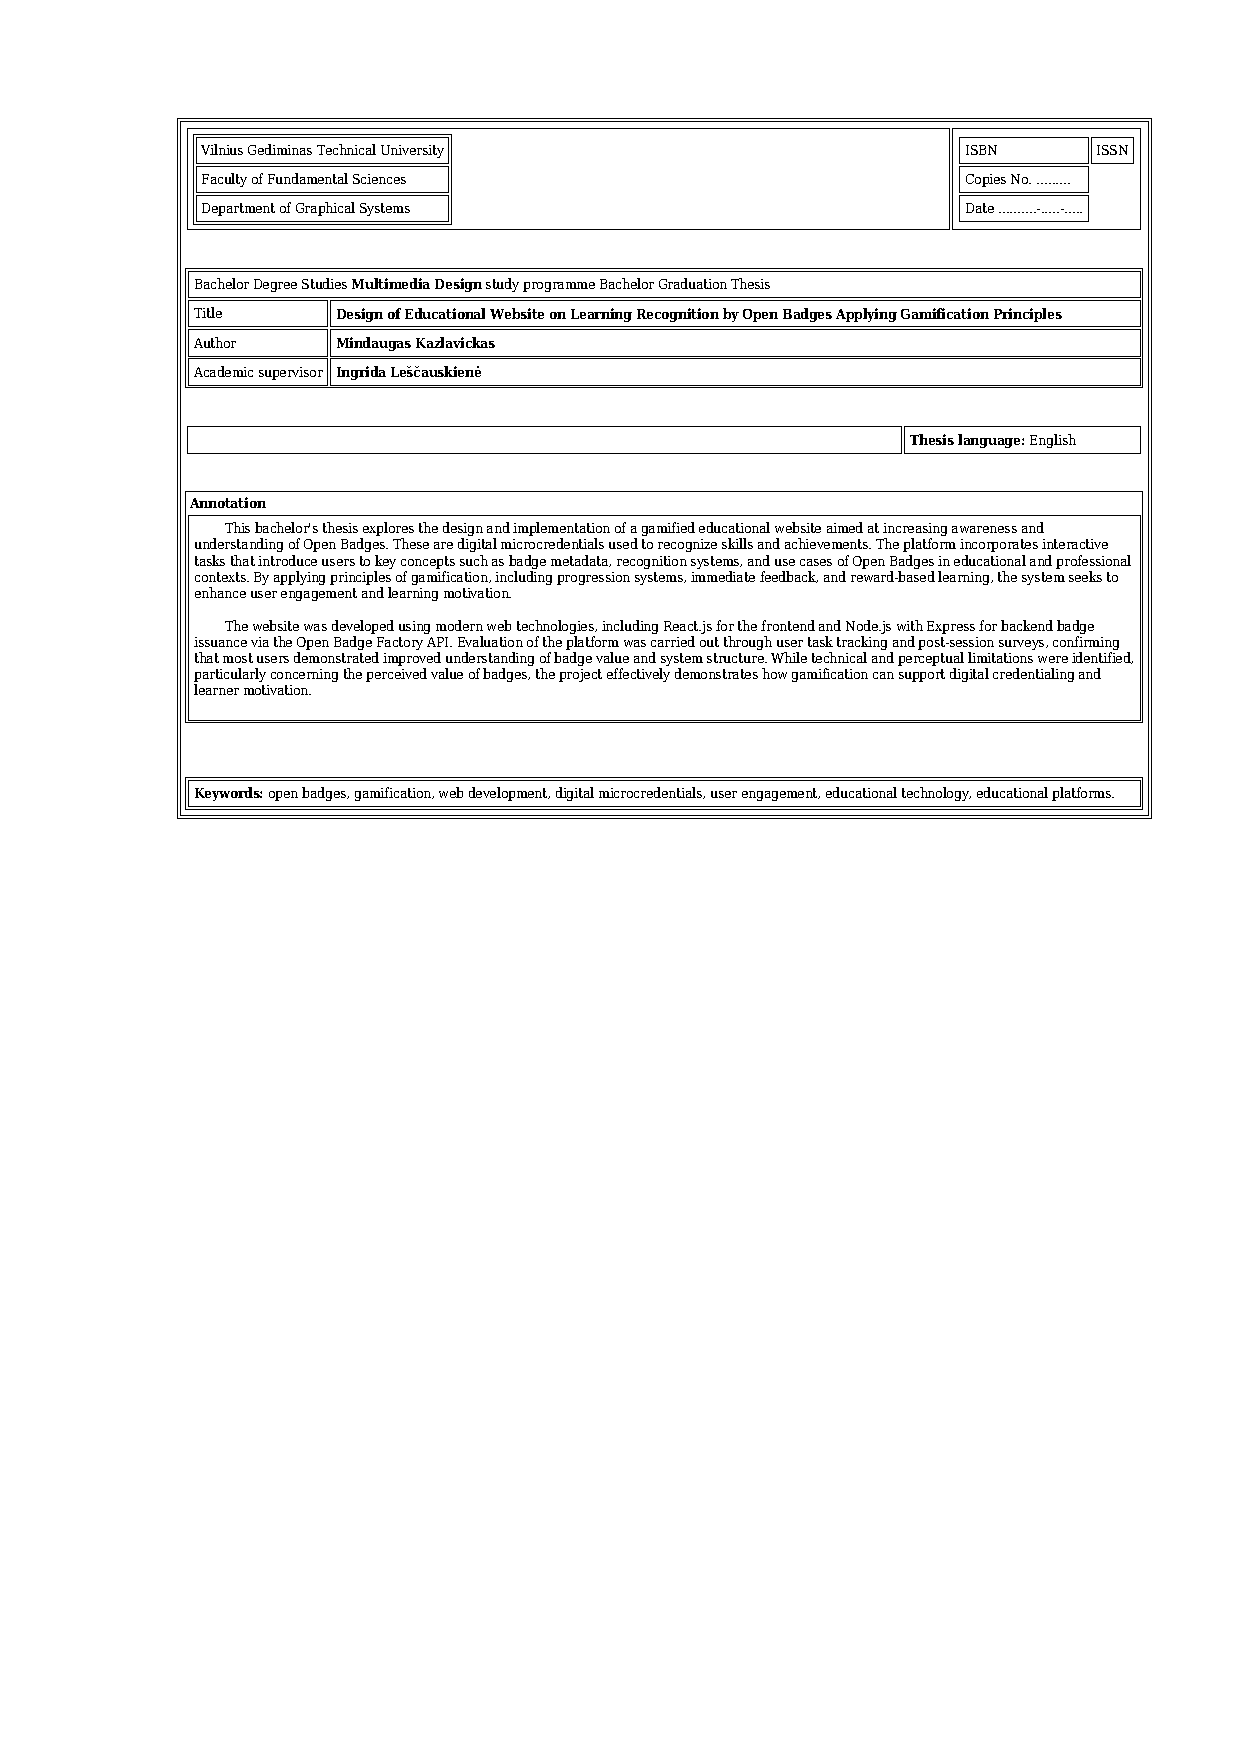
\includepdf[pages=-]{Files/annotation_en_Mindaugas.pdf}
\newpage
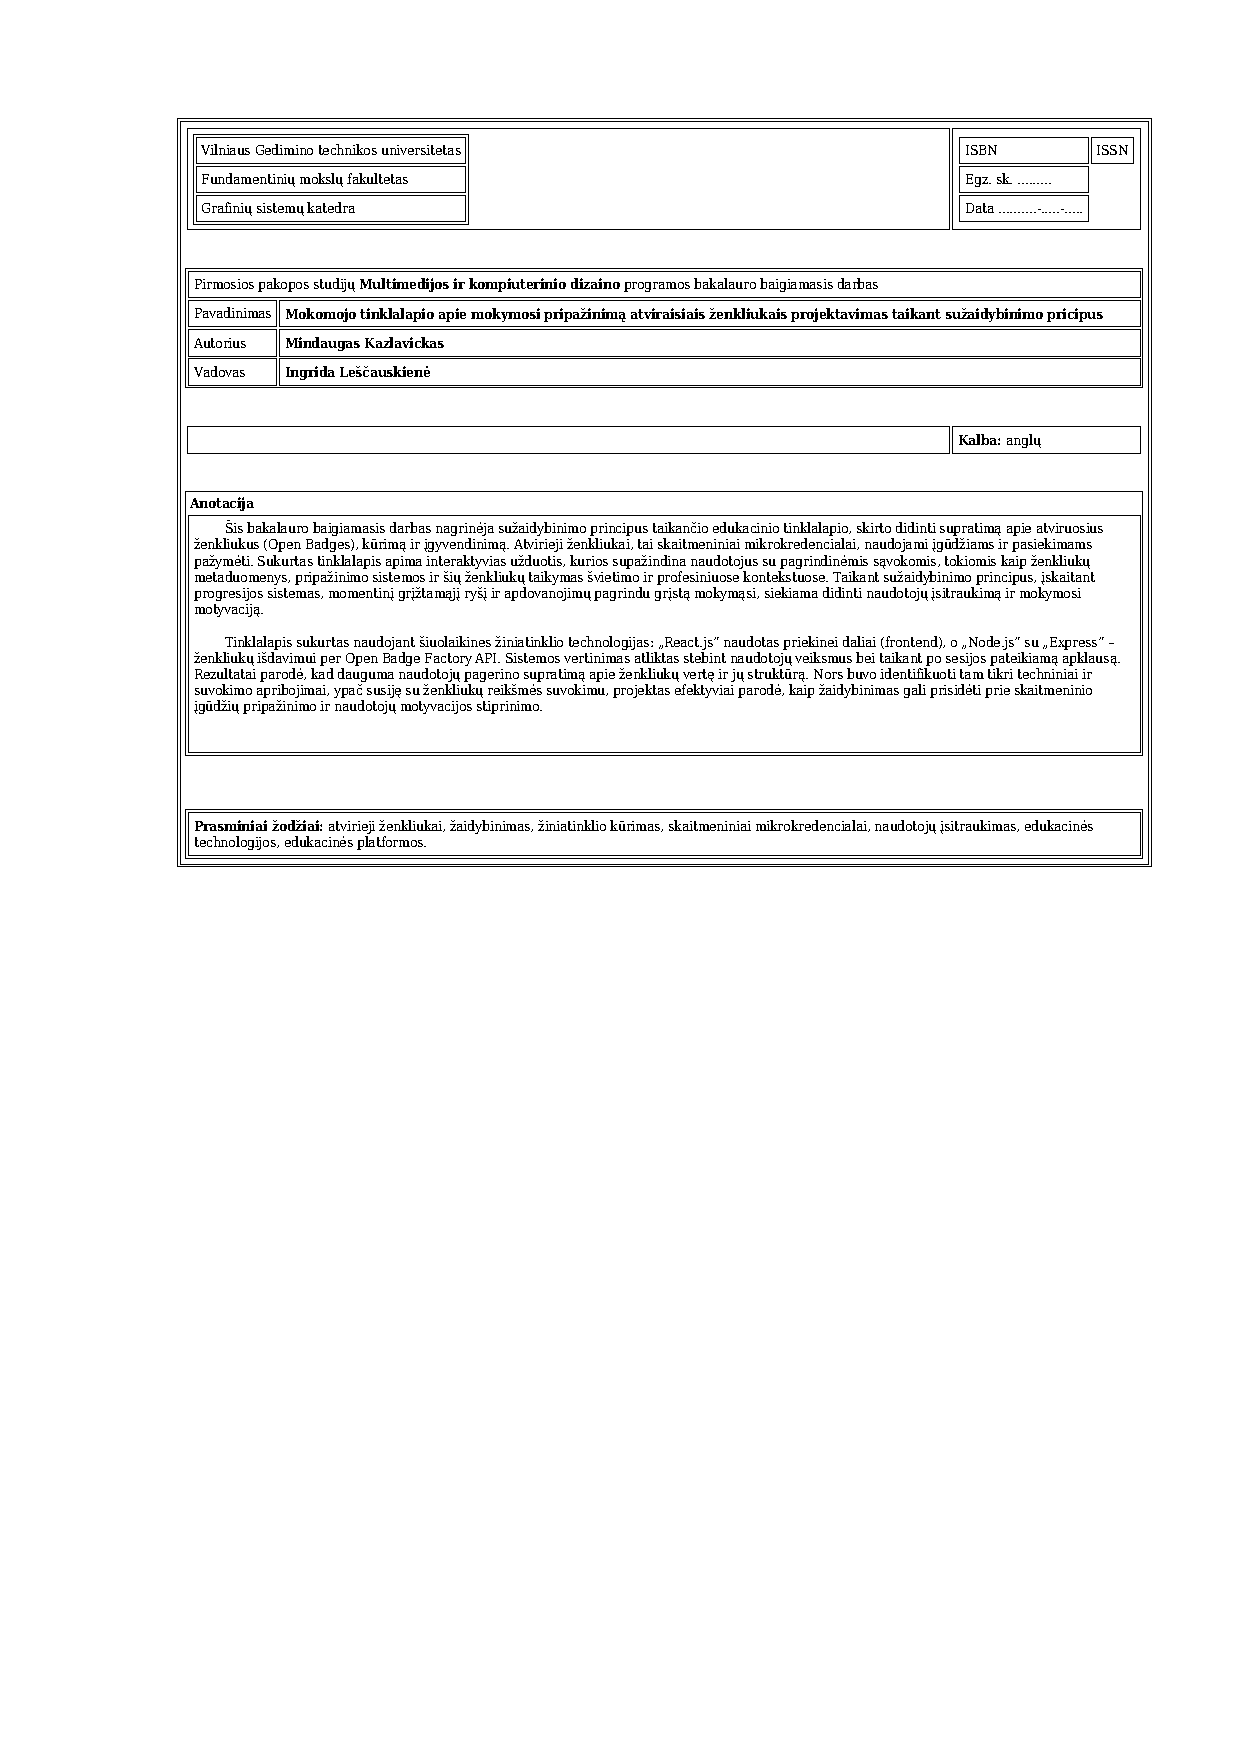
\includepdf[pages=-]{Files/annotation_lt_Mindaugas.pdf}
\newpage
%
\printglossary[type=acronym, title={List of Abbreviations}] % Abbreviations
\newpage
\tableofcontents    % Table of Contents
\newpage
\listoftables       % Tables
\newpage
\listoffigures      % Figures
\newpage
\clearpage
\listofloa          % Appendices
\newpage
%
\section*{INTRODUCTION}
\addcontentsline{toc}{section}{INTRODUCTION}
%
\textbf{Relevance of the topic.} The increasing focus on holistic education highlights the significance of recognising extracurricular achievements alongside academic credentials outside of the academic environment. 
Digital badges provide a flexible system for tracking and validating non-formal learning, offering students, staff and other participants an opportunity to articulate their skills effectively. 
Unfortunately, existing implementations fall short of engaging users and demonstrating the relevance to industry recruiters and evaluators who are responsible for incorporating these badges into industry practices.

Research \cite {Stefaniak_and_Carey} suggests the potential for open badges to foster confidence. 
Similarly, research \cite{definition}, \cite{nicholson2015} further advocates for meaningful gamification as a mechanism to enhance user involvement and long-term motivation with these systems to lead to lasting personal benefits.

By analyzing the environment of the application, and addressing gaps in awareness to improve engagement and practical implementation, this project aims to contribute towards gamified educational tools and their role in fostering self-determination, lifelong learning and further recognition of gamified systems. 
The project is concerned with the Vilnius Tech Open Badge System and for the purposes of the work, the core audience from this point will be considered higher education students.

\textbf{Problem -} The current systems for tracking extracurricular achievements lack robust user engagement strategies and fail to appeal to industry specialists as a form of credibility.
This disengagement often leads to user fatigue, frustration, and underutilization \cite {FunaAndAaron}. 
Consequently, some students who may struggle to recognize and articulate their skills are limiting their professional growth due to this underutilization.
Additionally, due to limited awareness, and recognition struggles \cite {federalIssues}, it is difficult to present them as appealing alternatives to recruiters.

\textbf{Research Object -} A gamified educational website-browser game that integrates a digital badge system to promote the recognition of open badges.

\textbf{Aim -} To develop an interactive, user-friendly educational website-browser game that uses gamification to showcase the value of open badges, facilitating recognition within the industry and aiding in the articulation of users’ skills and achievements.

\textbf{Tasks:} 
\begin{enumerate}
  \addtolength{\itemsep}{-0.5\baselineskip} 
  \item Analyze theoretical foundations of digital badges, gamification, and their application in education to identify best practices.
  \item Define technical and functional requirements for a gamified educational platform tailored to user engagement.
  \item Develop a prototype platform incorporating gamified elements that educate users about the badge system and its applications.
  \item Test and evaluate the prototype to assess user engagement and understanding of the badge system.
\end{enumerate}

\textbf{Research Methods:}
\begin{enumerate}
  \addtolength{\itemsep}{-0.5\baselineskip} 
  \item Literature Review: Conduct a focused review of existing research on gamification, digital badge systems, and their use in educational contexts to inform the platform's design, both from a theoretical and technical perspective.
  \item Prototype Development: Utilize the Phaser 3 game engine and modern web technologies to create an interactive and scalable platform.
  \item Evaluation: Explore testing possibilities, applications, and suggest future research and developments within the fields of gamification.
\end{enumerate}

Notably, this thesis is an extension of a previously completed academic report \cite{me2024}, "Gamification in Web Development".
\newpage
\newpage
\section{LITERATURE REVIEW}

Firstly, core definitions have to be established for key concepts to provide a foundational and universal understanding, followed by in-depth analysis of gamification  aspects and theories to achieve the desired results.

\begin{enumerate}
  \addtolength{\itemsep}{-0.5\baselineskip} 
  \item Gamification and Digital and Open badges.
  \item Gamification Aspects, Game Elements
\end{enumerate}

Definitions will be drawn from existing research works and recent studies to capture historical evolution and contemporary perspectives. 
After establishing the terminology, core aspects relevant to the project will be identified - user engagement with gamified systems, motivation, and the integration of gamified systems in educational settings and web spaces. 
This will be done with the goal of exploring their role in fostering self-determination, enhancing learning outcomes, and improving user adoption. 
Finally, critical elements for the success of the browser game are to be established for achieving the goal of the project.

%
\subsection{Establishing Core Concepts}

\subsubsection{Gamification}
%
The term itself was coined by Nick Pelling in 2002, who used it to describe the use of "game-like accelerated user interface design to make electronic [ATM vending machine] transactions both enjoyable and fast" \footnote{https://nanodome.wordpress.com/2011/08/09/the-short-prehistory-of-gamification/}. 
The greater academic exploration of gamification began around the 2010s, with researchers like Deterding and others formalizing the concept as the incorporation of game-like design elements, which aim to leverage intrinsic human motivations, into non-game contexts \cite{definition}.
Early 2010s definitions of gamification often reflect a similar focus on game mechanics - Kapp (2012)defines gamification as "the use of game thinking to engage people, motivate action, and promote learning"\cite{definition2}.

In contrast, later definitions such as Huotari and Hamari (2017) provide a more nuanced approach to the topic, describing gamification as "a process of enhancing a service with affordances for gameful experiences in order to support users' overall value creation"\cite{redefinition}.
This definition broadens the scope beyond individual game elements, focusing on how gamification can achieve a much more nuanced effect on people. 
And not without good reason, as recent statistics find gamification to increase engagement in online learning platforms by 90\% \footnote{https://review42.com/resources/gamification-statistics/\_gl=1*9edevd*\_gcl\_au*NTMyNzk5MTM3LjE3MjI1NDA5NTc.} leading to the understanding of why so many platforms today are proudly applying a gamified approach to education, such as Brilliant.org, Duolingo, Khan Academy and others finding great success. 
Another contrasting view is presented by Zichermann and Cunningham (2011), who argue that gamification can sometimes lead to superficial engagement if not aligned with intrinsic user motivations. 
They suggest that without a deep understanding of the target audience's needs, gamified elements might fail to produce meaningful engagement or long-term behaviour change\cite{bookOnEngagement}. 
The critique highlights the potential pitfall of applying gamification indiscriminately and stresses the importance of aligning gamification strategies with user motivations and context. In regard to user qualities, in \ref{fig:gamifiedVSnongamified} we can see a study result which found that introverted students will tend to engage with gamified systems more than extroverted students - introverted students have a higher correlation with progression and achievement within the gamified system, based on research by Smiderle et al\cite{gamifiedChart}.\\
\begin{figure}[htbp]
 \centering
 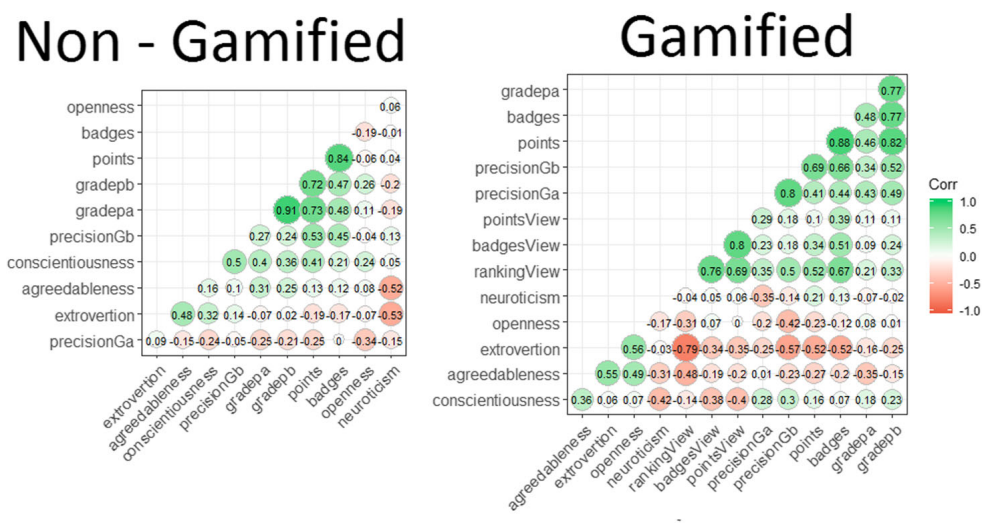
\includegraphics[width=\textwidth]{Media/chart.png}
 \caption{Correlogram for the relationship between all variables of the experiment}
 \label{fig:gamifiedVSnongamified}
 {\raggedright \small{Source: Smiderle et al., 2020}\par}
\end{figure}
Drawing from foundational definitions by Pelling (2002), Deterding et al. (2011), and Huotari and Hamari (2017), the analysis will focus on gamification as a tool to foster engagement, motivation, and learning outcomes with content or system.

In summary, gamification has proven to be a versatile and impactful strategy across various domains, supported by empirical evidence demonstrating its ability to enhance engagement, motivation, and learning performance. 
This scientific backing underscores the potential of gamification to transform user experiences and drive behaviour through the strategic application of game design principles.\\
%
\subsubsection{Digital and Open Badges}

Digital badges - visual representations of skills, achievements, or competencies earned by individuals through various learning or professional activities. 
This concept harkens back to traditional merit badges, that signify accomplishments in a tangible form, such as those awarded in organizations like the Boy Scouts. 
However, digital badges expand upon this concept by using technology for verification and credibility.

Research by Gibson et al. (2015)\cite{GibsonBadges} indicates that digital badges appeared in literature around 2010, which suggests a scarcity of comprehensive literature on the topic. 
The definition used for digital badges was "electronic representations of achievements or skills...", which matches the definition of traditional badges. 
It is however followed with "...including metadata that verifies the awarding body and the context of the achievement." 
This suggests that metadata is the core difference between the traditional and the digital - it contains essential information about the issuer, criteria for earning the badge, and evidence supporting the achievement. 
This transparency enhances their credibility and utility across various contexts (Bowen and Thomas, 2014)\cite{Bowen02012014}.

The first notable project with digital badges is considered The Mozilla Open Badges project, launched in 2011, as it created a standardized framework for their design, issuance, and verification\footnote{https://support.mozilla.org/en-US/kb/mozillas-open-badges-project}. 
This initiative allowed badges to be shared across platforms and promoted their recognition in educational and professional environments (Casilli \& Hickey, 2016)\cite{credentialsBadges}.

Such new functionality was immediately appealing for adoption within educational contexts to more effectively and verifiably recognize informal learning, complementing traditional academic credentials. 
According to Abramovich et al. (2013)\cite{areBadgesUseful}, they are motivational tools that provide learners with tangible evidence of their achievements. 
Furthermore, their ability to integrate gamified elements—such as progression systems, competition and reward structures—aligns them with broader trends in educational innovation. 
Recent studies indicate that incorporating badges into online courses can lead to higher completion rates and improved learning outcomes\cite{higherRates}.\\
{Digital Badge Characteristics}
%
\begin{figure}[htbp]
 \centering
 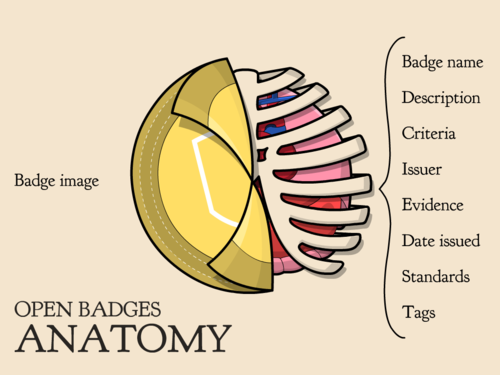
\includegraphics[width=14cm]{Media/OpenBadgeAnatomy.png}
 \caption{Open Badge Anatomy}
 \label{fig:badgeAnatomy}
 {\raggedright \small{Source: Awero team, badgecraft.eu, 2024}\par}
\end{figure}
%
\begin{enumerate}
  \addtolength{\itemsep}{-0.5\baselineskip} 
  \item Visual Symbols: Graphical representations that signify the type of achievement, skill or progress within a field. 
  This allows for easily identifiable information about the owner of the badge.
  \item Metadata-Enhanced: Each badge includes metadata that provides information about the issuer, potentially the criteria for earning the badge, as well as evidence of achievement in the form of uniquely trackable data. 
  An example anatomy is shown in \ref {fig:badgeAnatomy} \footnote{https://www.badgecraft.eu/en/blog/open-badges/understand-badge-meta-data}. 
  In all cases, the badge name, description and criteria are mandatory with the rest being optional.
  This metadata ensures transparency and helps validate the badge's significance.
  \item Portable Credentials: Badges can be easily shared across platforms such as social media, professional networks like LinkedIn, and personal websites. 
  This invites for quick transferability of verifiable information. 
  Notably, since badges represent primarily informal learning, as of writing this work, they do not inherently compete with professional networks and are intended as an extracurricular display of interests or abilities rather than professional or academic prowess.
\end{enumerate}

%
Both open badges and digital badges are forms of online credentials that signify skills, achievements, or competencies. 
However, there are significant differences in their frameworks. The key areas separating the two:
\begin{enumerate}
    \addtolength{\itemsep}{-0.5\baselineskip} 
  \item {Standards.} Using the framework created by the Mozilla Open Badges Project, a set of criteria is in place regarding the creation, issuance and verification of badges. 
  According to Young, West, \& Nylon (2019)\cite{whatIsAnOpenBadge}, for a badge to be classified as an open badge, it must be portable, shareable, controllable, and verifiable by both the issuers and the earners. 
  This standardization is in place to ensure that open badges carry metadata that provides comprehensive information about the learning experience, including badge criteria, issuer details, and evidence of achievement. 
  In contrast, general digital badges do not necessarily follow these standards. 
  Some digital badges are proprietary to specific platforms or institutions and may lack the metadata for multi-platform verification. 
  This inconsistency limits their broader adoption and recognition across different educational and professional contexts (Abramovich et al., 2013)\cite{areBadgesUseful}.
  \item {Interoperability.} It is critical to open badges as it allows for multi-platform utility and industry-crossing recognition. 
  It essentially allows for open badges to be portable. This portability allows individuals to showcase their achievements in diverse contexts and facilitates recognition by potential employers or educational institutions (Casilli \& Hickey, 2016)\cite{credentialsBadges}. 
  This is achieved by readability and adaptability which allows for universal recognition across the internet. 
  On the other hand, the lack of interoperability with normal digital badges hinders the ability to present them outside of proprietary platforms, greatly limiting their viability(Gibson et al., 2015)\cite{areBadgesUseful}.
  \item {Accessibility.} Open badges promote inclusivity by democratizing credentialing systems. 
  They enable learners or other forms of participants to earn recognition for achievements gained through informal learning experiences, volunteering, workshops, organization and more according to \footnote{https://digitalpromise.org/2023/04/13/the-relationship-between-digital-badges-and-micro-credentials/}Marilys Galindo and Casilli and Hickey \cite {credentialsBadges}. 
  The open nature of these badges allows for a more equitable representation across diverse fields. 
  In contrast, traditional digital badges may not provide the same level of accessibility. Basic digital badges may fail to meet system criteria, which creates a disparity and highlights the importance of adopting open badge frameworks to ensure all badge earners have equal opportunity. (Young et al., 2019)\cite {whatIsAnOpenBadge}. 
\end{enumerate}

\subsubsection{Criticism of Digital and Open Badges}
Despite the increasing value and application within educational and professional settings, open badges have received criticism, primarily regarding their potential to overemphasize extrinsic motivation at the expense of intrinsic learning. 
Risquez et al. (2020)\cite{risquez2020badge} argue that an exaggerated focus on external rewards, such as badges, can shift learners' priorities from acquiring knowledge to earning a reward. 
This phenomenon aligns with Deci and Ryan’s (1985)\cite{sdt} \acrshort{sdt}, where intrinsic motivation is necessary for sustained engagement and meaningful learning. 
When learners focus on achieving external markers of success, such as badges, their motivation to genuinely master content may diminish, and reduce the long-term impact on their educational process.

Research suggests that while digital badges can encourage learners to complete specific tasks, this form of external motivation does not consistently incentivize deeper cognitive engagement or subject mastery (Abramovich et al., 2013)\cite{areBadgesUseful}. 
For instance, the study by Casilli and Hickey (2016)\cite{credentialsBadges} found that while badges could lead to higher short-term task completion, their effectiveness in promoting improved thinking skills or critical analysis was not as improved. 
This highlights the importance of designing badge systems that complement, rather than replace, pedagogical strategies aimed at intrinsic motivation. 
A similar problem is of note within the Vilnius Tech Open Badge System, as a significant number of participants are more focused on the completionism of their badge collections rather than true extrinsic learning to present in the future.

While some forward-thinking organizations have begun to view badges as credible indicators of skill proficiency(examples as seen in chart \ref{fig:badgeExamples} \footnote{https://iite.unesco.org/highlights/open-badges-new-opportunities-to-recognize-and-validate-achievements-digitally/}), the majority continue to favor traditional credentials, such as degrees, certifications and professional media sites (Casilli and Hickey, 2016)\cite {credentialsBadges}. 
This undermines the potential of badges as a new force in skill recognition and professional development. 
Employers and educators remain sceptical of badge validity due to inconsistencies with digital badges used proprietarily instead of open badges, further exacerbating this issue.

\begin{figure}[htbp]
 \centering
 
\includegraphics[width=14cm]{Media/Open_badges_examples.png}
 \caption{Open Digital badges}
 \label{fig:badgeExamples}
 {\raggedright \small{Source: UNESCO Institute for Information Technology in Education, 2020}\par}
\end{figure}
Finally, the implementation of digital or open badge systems presents logistical and resource-related challenges, especially for institutions with limited budgets or technical expertise. 
As Gibson et al. (2015)\cite{GibsonBadges} point out, establishing a comprehensive badge ecosystem requires significant investment in technology infrastructure, staff training, and the development of mechanisms to ensure badge integrity. Smaller institutions, may struggle to allocate the necessary funds and manpower, limiting the adoption of digital and open badges across educational and professional environments.

Digital and open badges serve as innovative tools, but while their potential for motivating learners and complementing traditional credentials is promising, challenges such as overemphasis on extrinsic motivation, inconsistent recognition, and resource-intensive implementation limit their broader adoption. 
Addressing these issues could be the way for badges to transform educational and professional environments, promoting equitable and credible skill recognition.\\
%
% ------------------------------------------------------------------- SKYRIUS --
\subsection{Gamification Background Analysis}
%
\subsubsection{Psychology in Gamification}

Gamification is deeply rooted in psychological principles, significantly influencing behaviour and engagement. 
One of the core theories behind the psychology of gamification is Deci and Ryan's \acrshort{sdt}, \cite{sdt}which states that individuals are motivated by the need for competence, autonomy, and relatedness. 
These needs are leveraged by gamified systems by providing users with challenges (which lead to competence), choices (suggesting autonomy), and social interaction opportunities (relatedness). 
Research by Mekler et al. (2017) \cite{MEKLER2017525}demonstrates that satisfying these psychological needs through gamification can lead to improving performance quantity. 
For instance, leaderboards and achievement badges - both systems widely adapted outside of typical games, have found great success on digital platforms fulfilling their needs for personal, learning and health improvement. 
Examples include Duolingo, Brilliant.org and Nike's or Garmin's physical activity apps respectively, all of which lead to the user improving, by "choosing" to do so while competing with friends, family circles as well as platform communities. 
Providing users with choices in how they navigate a journey of self-improvement increases the sense of motivation for the users as all of the aforementioned platforms actively apply \acrshort{sdt} in their approaches.

Another critical psychological aspect that is core for gamification is the concept of flow, introduced in 1990 by Csikszentmihalyi \cite{flow}. 
Flow is the state of deep immersion and focus, where individuals lose track of time and are fully engaged in an activity. 
Gamification easily facilitates such a state by creating well-balanced challenges that are neither too easy nor too difficult, thus maintaining peak user interest and engagement. 
These psychological principles are strategically applied to drive desired behaviours. 
For example, Duolingo and Codeacademy.com employ progress tracking of multiple types, as seen in chart \ref{fig:duolingoProgress}, rewards, and social competition as well as adaptive difficulty challenges and a choice of studies or languages to learn, that way keeping users motivated and engaged, demonstrating a practical application of \acrshort{sdt} and flow theory.

\begin{figure}[htbp]
 \centering
 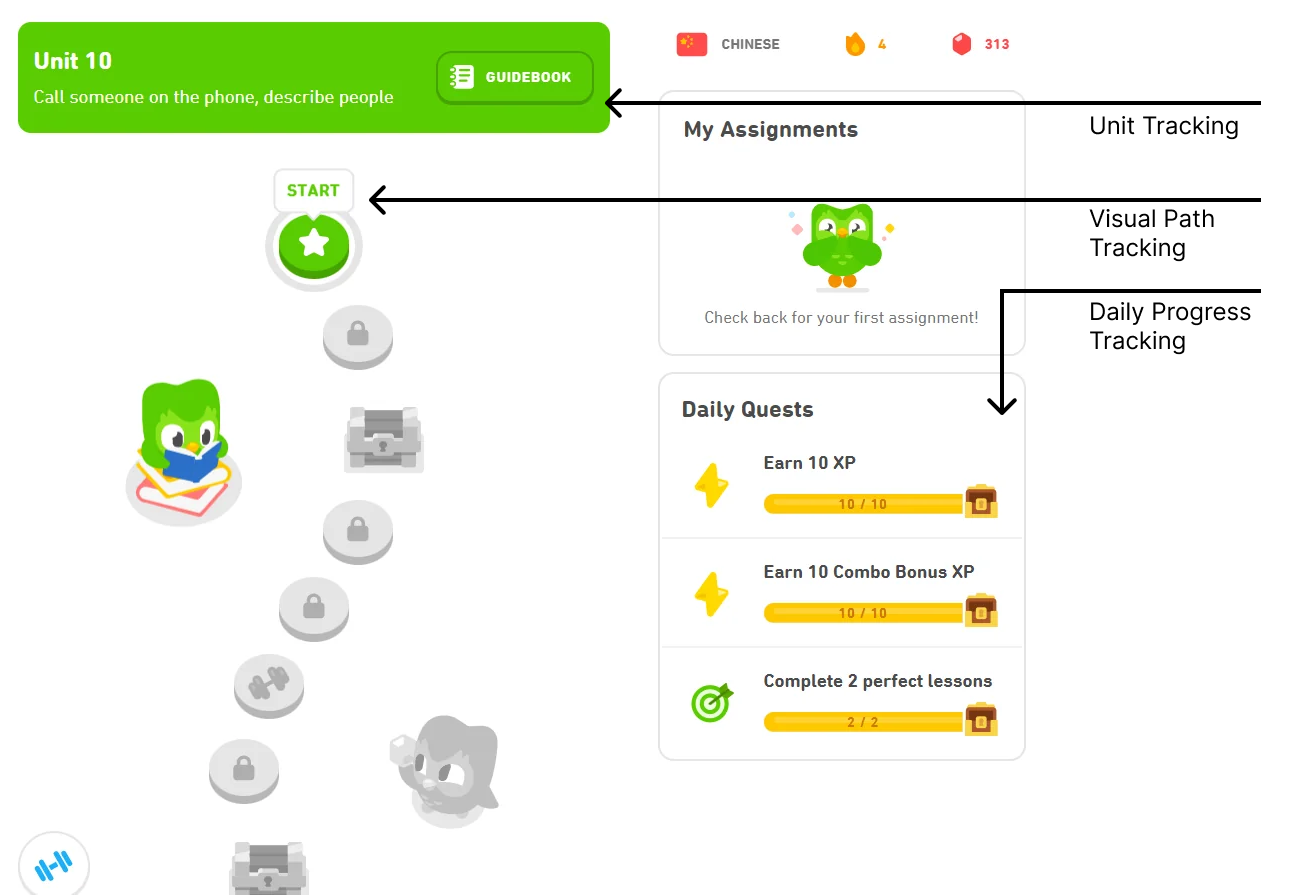
\includegraphics[width=14cm]{Media/DuolingoProgress.png}
 \caption{Various types of Duolingo progress tracking}
 \label{fig:duolingoProgress}
  {\raggedright \small{Source: Duolingo for desktop, 2024}\par}
\end{figure}

However, some research also suggests that while gamification is an excellent engagement boost, especially through social influence, it may not be a guaranteed information retention or personal improvement enhancer, as in more quantitative studies, it was found that gamification only partially outperformed control groups in some areas\cite{doesItWork}. 
So according to Hamari and Koivisto (2015), while gamification can significantly boost user engagement and participation, improved results for the user are not inherent. 
The pitfalls of the application are the factors of the context that is being gamified as well as the qualities of the users. 
This is further supported by a study by Chernbumroong et al., where people were researched in a virtual reality museum, with either gamified or non-gamified systems in place. 
The gamified version left a much greater impression but negligibly improved information retention\cite{VR}. 
This suggests that while maintaining the engagement of the user in a learning context can lead to accelerated improvement, it is not guaranteed. 
This is not the case in areas where engagement is key. 
That is particularly relevant in marketing, where social proof, engagement, peer endorsements and attention retention provide excellent marketing opportunities and enhance brand loyalty, recognition and consumer trust through the exposition of products and services.

\subsubsection{Gamification in Marketing}

Gamification has become a valuable tool and has revolutionized marketing strategies by embedding game-thinking scenarios for the audience into brand interactions, thereby fostering greater customer engagement and loyalty\cite{redefinition}. 
One prominent example of gamification in marketing is the Sephora Beauty Insider program \footnote{https://loyaltylion.com/blog/scale-success-story-sephoras-beauty-insider}. 
The initiative leverages a tiered rewards system where customers earn points for various activities, which can then be exchanged for exclusive rewards. 
This approach not only promotes customer interaction but also encourages repeat purchases by offering tangible incentives. Moreover, gamification has proven effective in boosting brand visibility and recall. 
Robson et al. (2015) found that campaigns incorporating gamified elements tend to receive more shares on social media, thereby amplifying brand reach \cite{gameon}. 
For instance, McDonald's "Monopoly" promotion engages customers by allowing them to collect game pieces with each purchase \footnote{https://smartico.ai/mcdonalds-uses-gamification-boost-sales-retention/}. 
These pieces can be used to win prizes or traded, thereby increasing both brand exposure and consumer interaction.

Gamification facilitates immersive experiences that enhance customer engagement and loyalty. 
Hamari et al. (2014) observed that gamified features in loyalty programs, such as Starbucks Rewards, lead to improved user satisfaction and retention \cite{doesItWork}. 
The program’s use of points and badges motivates frequent interaction, resulting in increased customer spending and stronger brand relationships. 
Regarding badges, a study by Hamari (2015) suggested that badges are a great way to boost a system's usability but also that its engagement tends to decline with time\cite{badges}. 
Other challenges are also present according to Nicholson (2015), that highlight ineffective gamification strategies leading to superficial engagement, and failing to foster long-term loyalty or meaningful behaviour change \cite{nicholson2015}. 
Additionally, Robson et al. (2015) found examples of failed gamification approaches that happened due to no achievements or extrinsic rewards being offered for the user's performance within the intrinsic systems. 
Essentially, a poorly executed campaign that does not resonate with users' intrinsic motivations or provide substantial value may only achieve temporary engagement. 
\begin{figure}[htbp]
  \centering
  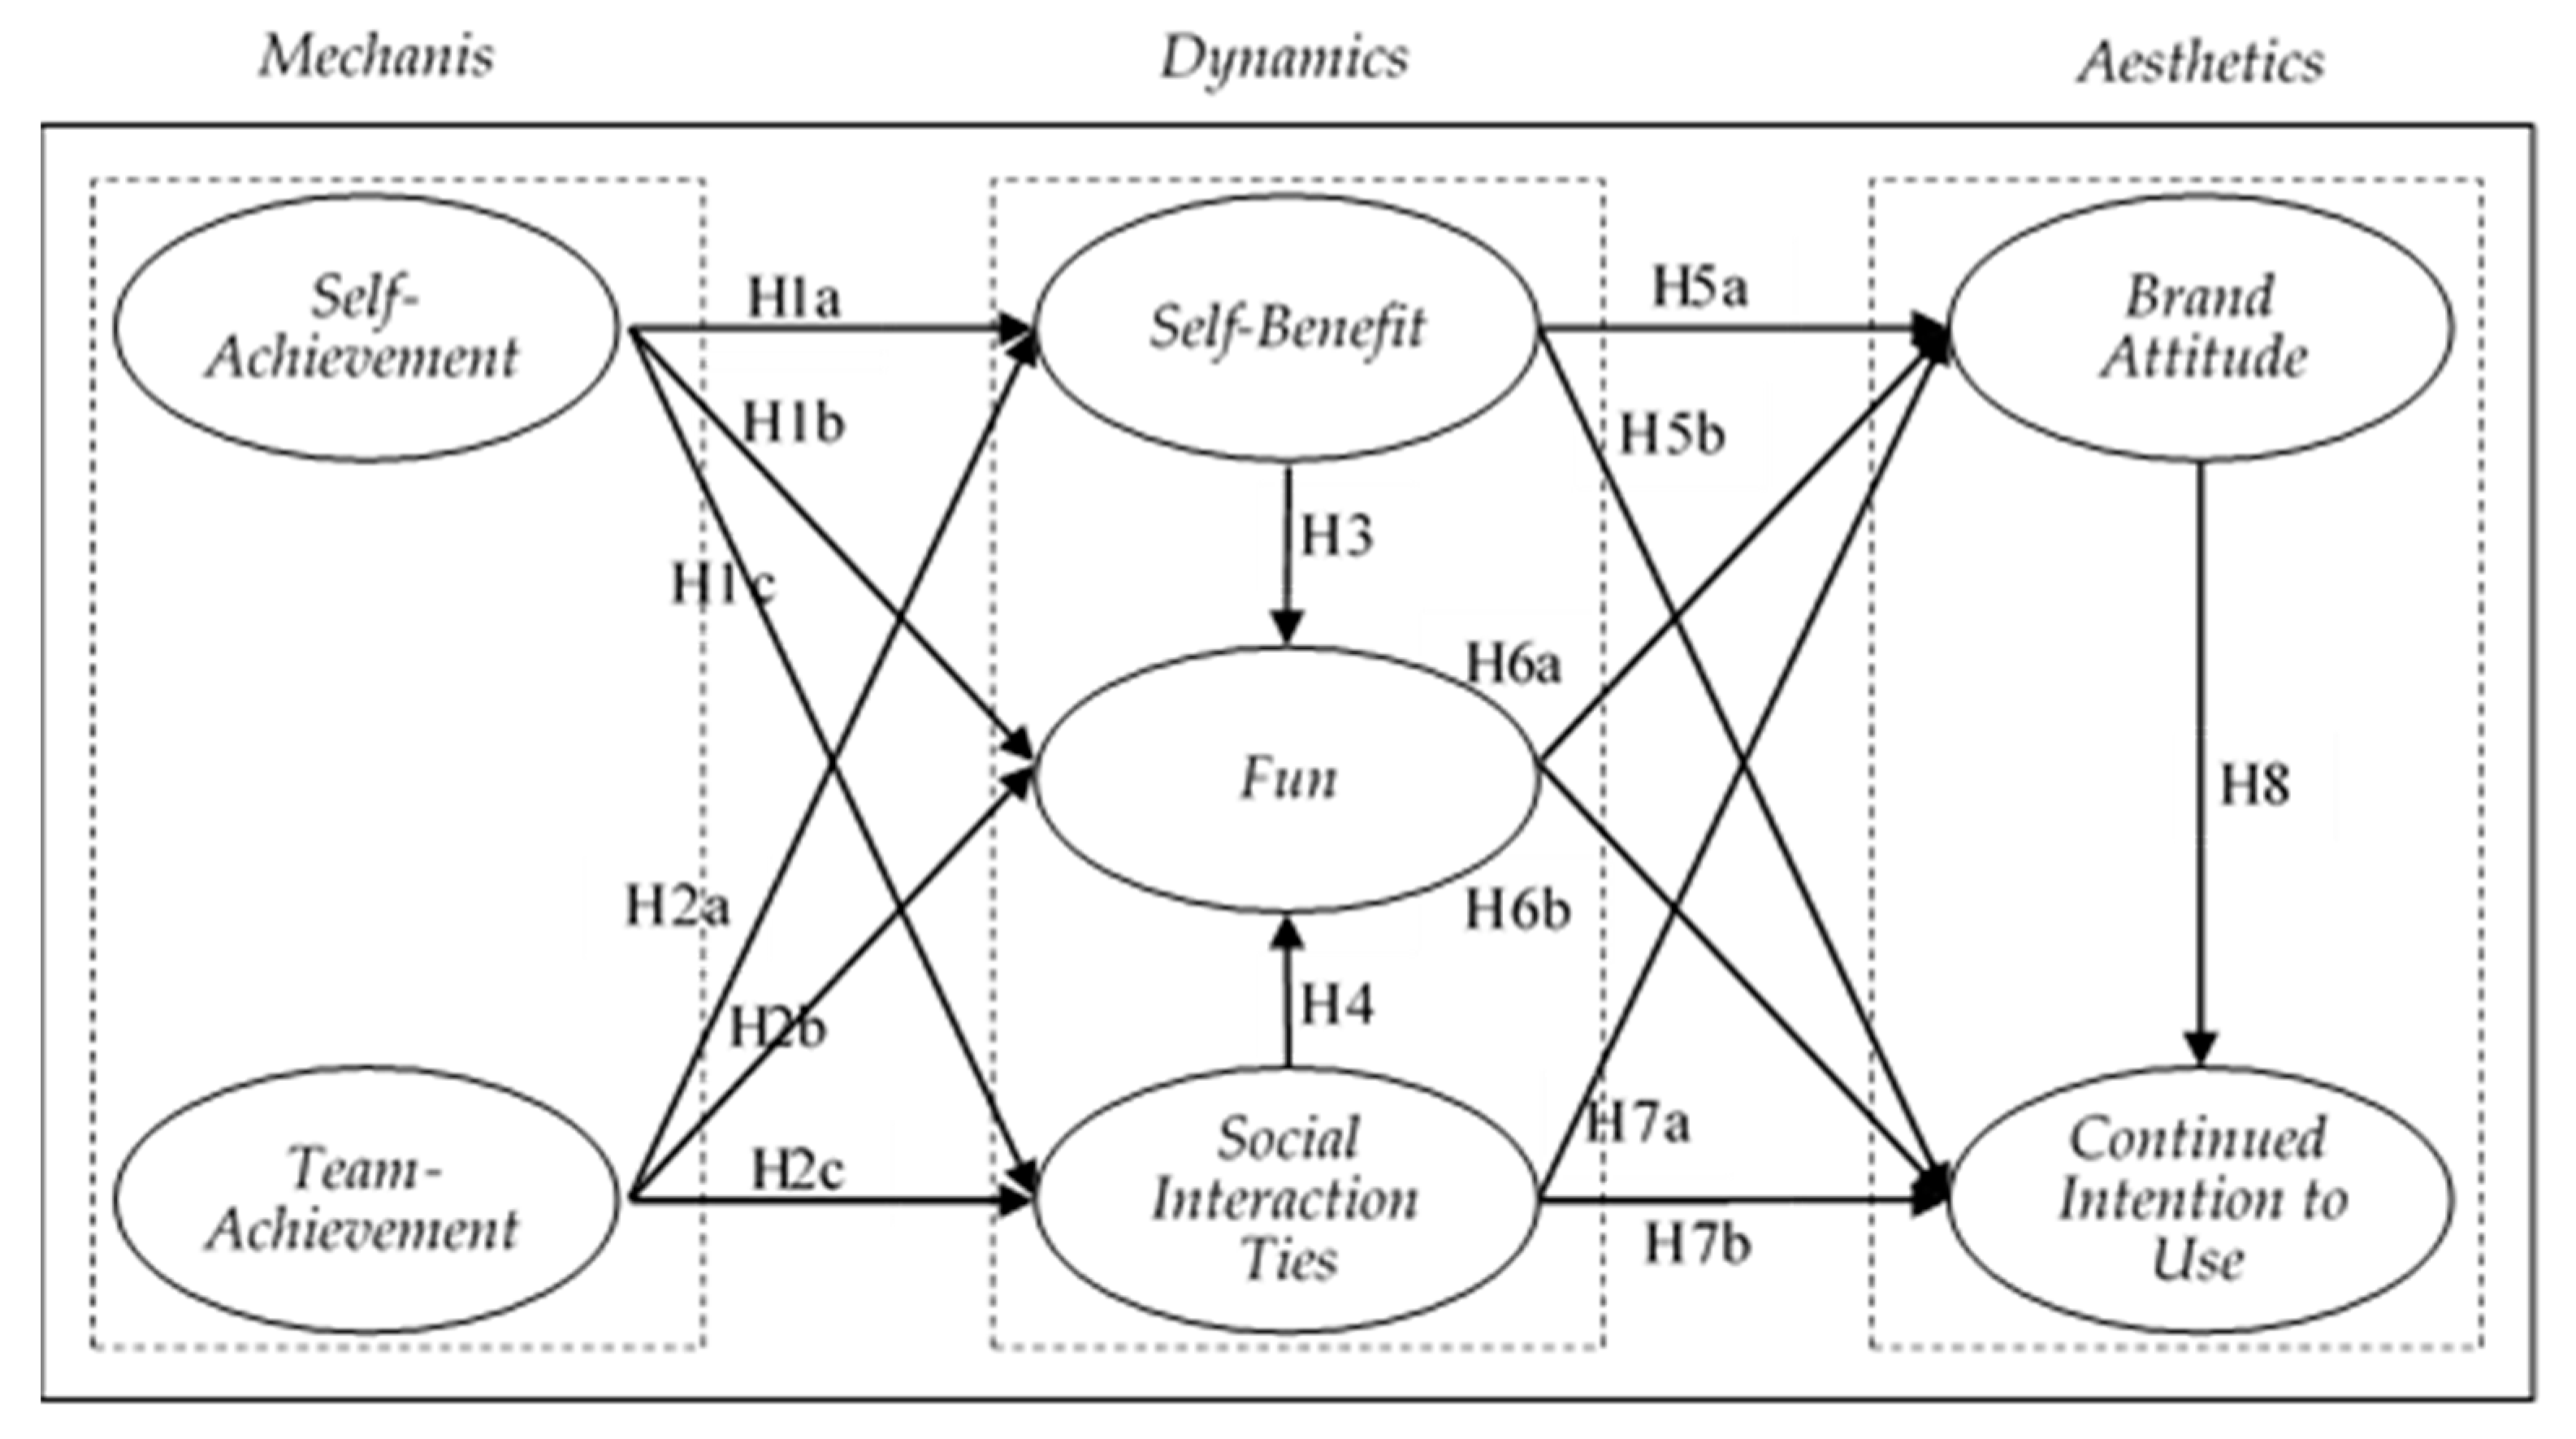
\includegraphics[width=\textwidth]{Media/sustainability2.png}
  \caption{Research model for the \acrshort{mda} framework}
  \label{fig:explainedDataChart}
{\raggedright \small{Source: Hsi-Peng Lu and Hui-Chen Ho, 2020}\par}
\end{figure}
Ensuring that gamified elements are well-aligned with user needs is crucial for sustaining engagement and maintaining a positive brand image.
Evidence from successful programs like Sephora’s Beauty Insider, McDonald's Monopoly and Starbucks Rewards underscore the effectiveness of gamification in marketing.

\subsubsection{Gamification in Web Development}

With web development adapting increasingly more techniques to endlessly growing user engagement, gamification has naturally become one of the pillars of its development. 
Research by Bitrian et al. (2020) shows that browser games can leverage all of the gamification benefits as well as feature very low entry barriers due to the web's accessibility and popularity \cite{roleOfMobile}. 
Additionally, Hamari et al. (2014) highlight that gamification solutions can substantially enhance software and service user engagement, a principle that applies effectively to browser games \cite{doesItWork}.

Lu and Ho (2021) explore how gamification affects user engagement in brand applications, demonstrating that gamified strategies can sustain user interaction and strengthen brand connections \cite{sustainability}. 
Games like "Cookie Clicker" employ progression systems and in-game economies to keep players invested and returning over long periods. 
Furthermore, a blog by Redacción Aguayo (2023) discusses various gamification strategies in digital product design, emphasizing their role in improving user experiences and driving engagement \cite{UXdesign}. 
Browser-based educational games like "Prodigy" use rewards and challenges to make learning more engaging, thereby increasing user satisfaction and retention.
Granted, most browser games exist within confined ecosystems like Facebook where they're meant to maintain engagement but solely to keep users terminally online as long as possible with examples like "Farmville".

To better understand the exact elements of gamification to apply in products and services, frameworks were designed to appropriately identify and apply resources to successfully gamify products. 
The most important success factor to achieve gamification of products, systems and services is "fun". 
The \acrshort{mda} framework to achieve "fun" applied by gamification according to research by Hunicke et al. consists of the following aspects\cite{sustainability}:

\begin{itemize}
    \item \textbf{Mechanics}:  The rules and systems that guide the gameplay.
    \item \textbf{Dynamics}:  The run-time behaviour of the mechanics, shaped by the players' interactions.
    \item \textbf{Aesthetics}:  The emotional responses or experiences the game evokes in players.
\end{itemize}

This provides a structured way to think about how different elements of game design come together to deliver an engaging experience. 
This is further expanded upon in \ref{fig:explainedDataChart}, which analyzes the relevant aspects of gamification through a study that tests specific applications of each aspect and how they affect each other to achieve marketing goals through a handful of hypotheses. 
An interesting finding within the study was that after measuring the results of the study, team achievements were least efficient in "fun" and end results, which leads to suggest that in spite of the importance of team-building or team-based exercises, team-based elements have to have complementary self-achievement to achieve desired results. 
The study was conducted by gamifying running exercises. 
Notably, the study found that continued usage and brand attitude is more important for newly acquired customers or people who are not yet customers. 
This indicates that gamification is much more efficient in acquiring new customers rather than retaining existing customers. 
Experienced or existing customers may have a different focus and preferences \cite{sustainability}.

These studies show that gamification, for a handful of purposes, has been in the web development space for a considerable amount of time by now and collectively it is focused on maintaining user engagement and compelling users to stay on relevant platforms and likely acclimate to provider services\cite{userEngagement}\cite{gamificationEngagement}.
%
\newpage
\newpage
\section{TECHNOLOGY REVIEW}

To achieve the goal of the work, necessary design, gamification and game elements have to be identified, to develop an educational website that applies gamification principles to teach and drive recognition for open badges. 
While there is no exact example in the industry to follow for achieving this task, existing solutions of education and gamification applied in learning, digital badge systems will be reviewed, highlighting their core gamification features, similarities, and theories applied.

To develop the task, technology and software solutions will be reviewed for the website. 
Finally, the completion of the website's content is intended to reward the user with an open badge of their own. 
This means that an open badge creation pipeline solution has to be explored, alongside metadata creation and its content to provide the website users with a token of verifiable completion that can be interoperably used across the Web.

\subsection{Review of Existing Similar Solutions}
Existing similar solutions will be reviewed to identify key features, gamified elements, and theoretical strategies relevant to designing them. For the purposes of the project, the only concern is with educational, gamification and open badge integrations. 
The analysis will focus on platforms utilizing features such as badges, progress tracking, and leaderboards and the approach to their design to identify key elements and features to be implemented. 
To provide depth, theoretical frameworks like \acrshort{sdt}, \acrshort{mda} Framework, flow theory and alternative approaches will be explored in their application to these platforms. 
This review will adopt a comparative analysis approach, organizing findings into four core criteria: platform name, gamification approach and features, theoretical foundations or strategies applied, and relevance to project goals. 
Aspects like Target Audience, Accessibility, strengths and weaknesses as well as many other potential outlines will be ignored due to being considered out-of-scope for the project. 
Additionally, the selected products and services to-be-reviewed vary significantly in scope and application, so expanding the set of criteria to evaluate would lead to misrepresentation of certain criteria aspects.
By examining how these solutions address engagement and skill recognition, the review aims to conclude elements and strategies to inform the design of a gamified educational website about open badges.

Chart Criteria
\begin{itemize}
    \item \textbf{Platform Name and Type}:  Identity of the tool or platform and the type it represents.
    \item \textbf{Gamification and Features}:  Highlight applied game elements such as badges, leaderboards, progress tracking. Additional features, most notably open badge support and creation.
    \item \textbf{Theoretical Foundations or Strategies Applied}:  Examine the applied academic or practical design principles used to develop the features, to ensure evidence-based practices.
    \item \textbf{Relevance to Project Goals}: Explore relevance of application to the work, specifically in the field of recognition of achievement, recognition and integration of open badges. This ensures that actionable features and strategies are identified.
\end{itemize}


\begin{longtable}[c]{|p{3cm}|p{4.2cm}|p{4.2cm}|p{4.2cm}|}
\captionsetup{justification=raggedright, singlelinecheck=false}
\caption{Comparative Analysis of Existing Platforms} \\
\hline
\textbf{Platform Name, Type} & \textbf{Gamification and Features} & \textbf{Theoretical Foundations or Strategies Applied} & \textbf{Relevance to Project} \\
\hline
\endfirsthead
\hline
\textbf{Platform Name, Type} & \textbf{Gamification and Features} & \textbf{Theoretical Foundations or Strategies Applied} & \textbf{Relevance to Project} \\
\hline
\endhead
\hline
\endfoot
\hline
\endlastfoot

\textbf{Mozilla Open Badges, Open Badge System} & Open badge creation, sharing, verification. Supports rich metadata, dictates international standards for issuing badges for educational accreditations. & Open recognition and learner autonomy principles, which tie into \acrshort{sdt}. The focus is on creating a standardized system for recognition, with an emphasis on verifiability and interoperability. & Provides the technical infrastructure needed to issue, verify, and share digital badges as well as the necessary metadata standards dictated. \\
\hline
\textbf{Badgr (Canvas Badges), Open Badge System} & Badge issuance, progress tracking, \acrshort{lms} integration, and social sharing options. & Use of badges, achievements and progress tracking aligned with \acrshort{sdt} and flow theory. & Supports easy digital badge creation, tracking of and rewarding learning achievements on manageable tracks, highly relevant for hassle-free digital badge creation. \\
\hline
\textbf{Open Badge Factory, Open Badge System} & Badge creation, issuing, and sharing, with reporting and data analysis features. & Encourages engagement through earning, tracking, and rewarding achievements. & Directly aligns with the goal of creating and recognizing open badges, offering a clear example of implementing badge metadata. \\
\hline
\textbf{Duolingo, Language Learning App} & Badges, streaks, Experience points, leaderboards, interactive lessons, various types of time-based, performance-based, task and progress tracking. & \acrshort{sdt} application - user autonomy, setup for achieving competence, relatedness through social systems, MDA Framework for driving engagement. & Engages users with gamified visual elements - badges, trackers, a map of Units. Supports skill recognition through milestones, suggests that having multiple ways of tracking progress is likely important for the user to keep track of their progress. \\
\hline
\textbf{Khan Academy, Educational Platform} & Progress tracking, mastery points, badges, personalized dashboards. & Mastery-based learning, flow theory for balanced challenges and skill levels. & Emphasizes clear progress indicators and personalized learning paths for user motivation. \\
\hline
\textbf{Coursera, Online Learning Platform} & Courses with progress tracking, certificates, community engagement. & Constructivist(enable users to construct their own understanding of the topic) learning, social learning, \acrshort{sdt} application for intrinsic motivation. & Combines certification and achievement systems, ideal for integrating open badges. \\
\hline
\textbf{Classcraft, Gamified Learning Platform} & Role-playing game mechanics (Experience, level-ups), collaboration, quests, and rewards. Includes avatars, team-based challenges, and behaviour tracking. & \acrshort{sdt} - focuses on competence through skill mastery, autonomy via customizable avatars and quests, relatedness through team-based interactions. & Encourages engagement and motivation through collaboration and role-playing elements, ideal for promoting both individual and group-based achievements. \\ \hline 
\textbf{Habitica, Task and Habit Tracker} & Gamified to-do list with tasks, streaks, and rewards. Users earn experience points and rewards for completing real-life tasks and goals. & \acrshort{sdt} application - intrinsic motivation through task completion and goal setting, competence through measurable progress, autonomy in managing tasks. & Provides a fun, gamified way to encourage habit formation and task completion, suitable for user achievement tracking in everyday activities. \\ \hline 
\textbf{Kahoot!, Game-Based Learning Platform} & Interactive quizzes, surveys, polls, leaderboards, and real-time gameplay in classrooms or teams. & Active learning principles, \acrshort{sdt} through engagement and social interaction in competitive settings. & Facilitates real-time, competitive learning, ideal for assessing knowledge and encouraging participation in educational settings. \\ \hline
\end{longtable}
{\raggedright \small{Source:} compiled by the author\par}

Platforms Mozilla Open Badges, and Open Badge Factory, which provide standardized badge creation and management systems are both viable options for issuing the work-related open badges for the purposes of the project. 
Badgr seems like a great addition that could go on to improve the experience with simple extra digital badges to explain the difference between digital and open badges. 
These systems align with the goal of the project for open recognition of the final badge and digital achievement recognition.

Gamified applications like Duolingo, Classcraft, and Habitica are focused on incorporating interactive elements such as streaks, quests, progress trackers and experience points to motivate users. 
By applying \acrshort{sdt}, these platforms effectively enhance intrinsic motivation through autonomy and competence (\cite{sdt}). 
Their emphasis on visual progress tracking and driving engagement highlights the importance of user-friendly interfaces for sustained participation. 
Duolingo’s gamified elements have been shown to increase user engagement and retention rates significantly.

Educational platforms Khan Academy and Coursera have developed personalized learning paths, mastery-based progress tracking, and social learning. 
These features are rooted in mastery learning, constructivist approaches, and active learning principles, which suggests the importance of personalized educational experiences that balance challenge and skill to maintain user engagement, per the flow theory (\cite{flow}, \cite{powerFeedback}). 
Unfortunately, personalizing learning paths and creating extensive social learning opportunities would not be viable for the project due to being considered out-of-scope for both aspects. 
Kahoot! and Classcraft emphasize collaborative and competitive learning, team-based interactions and real-time participation to encourage both individual and group achievements. 
While team-based interactions are also considered out-of-scope for the project, there is the opportunity to implement the playfulness of presenting educational content like they are done in both of these platforms to improve the user experience.

Overall, the findings suggest that combining the structured credentialing of open badge systems with the engaging, user-centric design of gamified platforms can create an intuitive framework for motivated learning. 
These strategies and practical insights will serve as the foundation for designing an educational platform that integrates gamification and achievement recognition to drive both user engagement and educational outcomes.

\subsection{Technology Review}

\begin{enumerate}
  \addtolength{\itemsep}{-0.5\baselineskip} 
  \item {Gamification and Motivation.} \acrshort{sdt}, flow theory and \acrshort{mda} will be applied for the design of the gamified website, in the forms of progress tracking, leaderboard (completion time) and rewards (the digital and open badges)(\cite{sdt}, \cite{flow}).
  \item {Open Badges and Digital Credentialing.} Digital badges will be created and issued using international metadata standards outlined by the Mozilla Open Badges. 
  A pursuit to create them through automatic means will then be made, whether with one of the available tools (Mozilla Open Badges, Badgr, Open Badge Factory).
  \item {User Experience and Interface Design.} A user interface will be implemented for user flow and driving user engagement. 
  The standard goal for the user interface will be a successful application of \acrshort{fbm} (\cite{fogg}), which is focused on three key factors: motivation, ability and triggers. 
  Simplicity is crucial to \acrshort{fbm}  to reduce friction and drive user engagement. 
  To further illustrate this, Figure \ref{fig:foggChart} \footnote{https://behaviormodel.org/} shows that specifically a balance of the three barriers is necessary. 
  So by making the platform more approachable and visually appealing, minimising barriers and using user-centric design, it is possible to improve learning follow-through.
  \item {Responsive Web Design.} The website will be designed mobile-first with relevant principles, as that is where most people are likely to experience the content according to \textcite{mobileDesign}. 
\end{enumerate}

\begin{figure}[htbp]
 \centering
 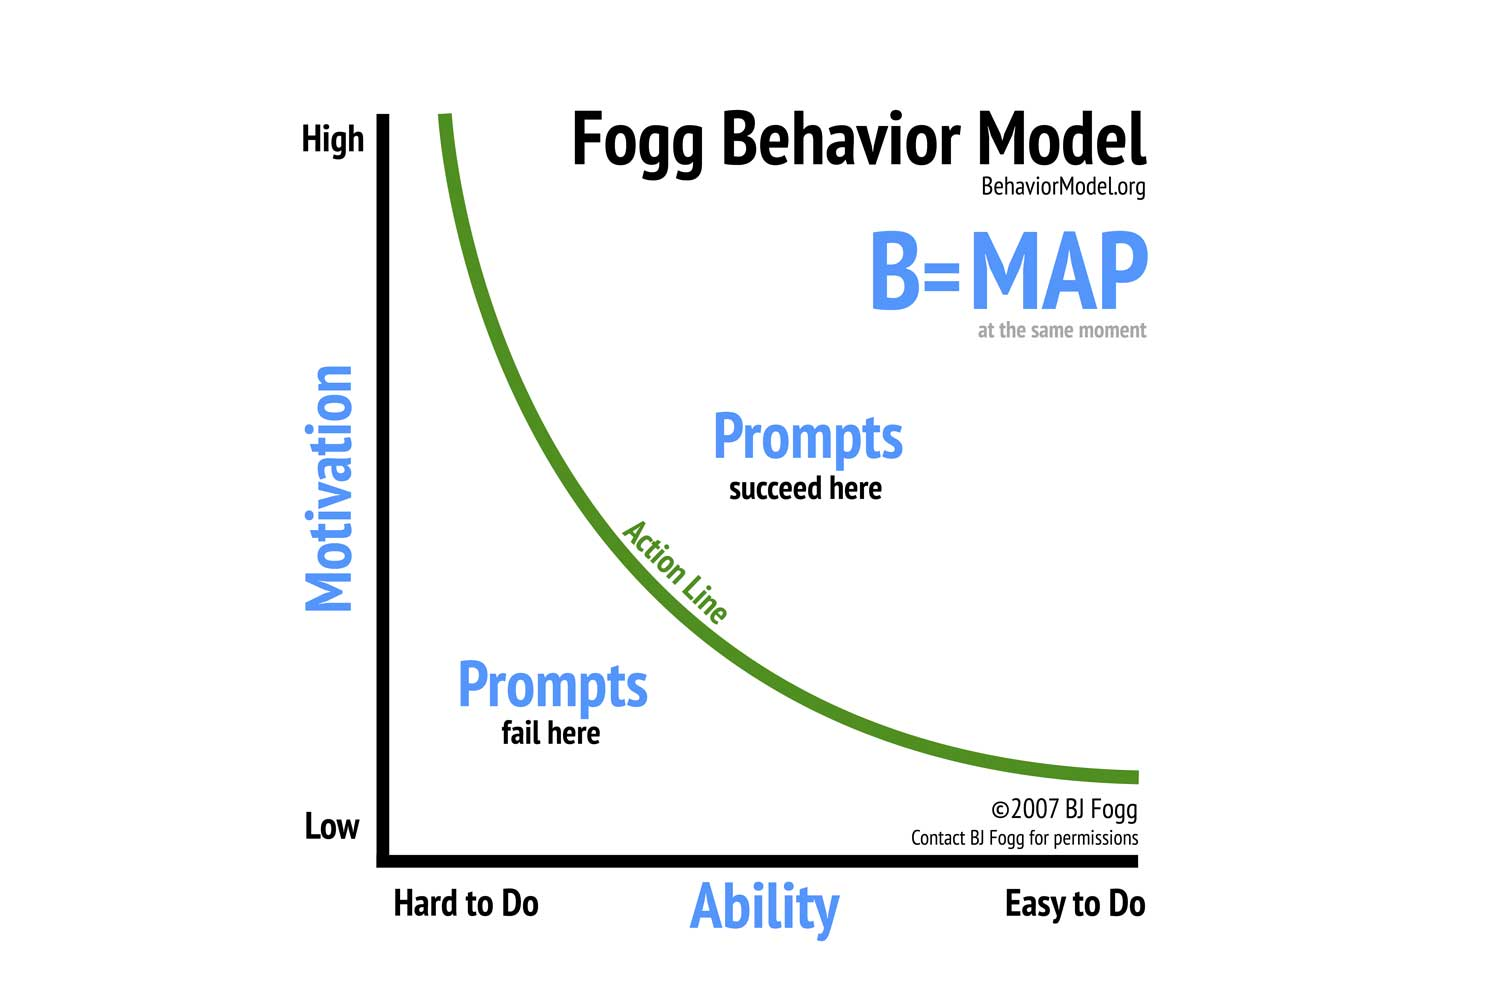
\includegraphics[width=14cm]{Media/Fogg-Behavior-Model.jpg}
 \caption{Fogg's Behavior Model}
 \label{fig:foggChart}
 {\raggedright \small{Source:} behaviormodel.org, 2009\par}
\end{figure}

\subsection{Website Characteristics Review}

\begin{enumerate}
    \item \textbf{User Engagement and Motivation:} 
    \begin{itemize}
        \item \textbf{Gamified Elements.}
        \begin{itemize}
            \item Progress bars and trackers. Progress trackers will be visible within tasks and between them so that users can clearly understand their current state and progress. 
            This will be implemented selectively for each task given to the user.
            \item Score system. Users will gain and lose points based on their performance, which will be submitted as part of their badge criteria.
            This will incentivize better analysis of the provided reading materials.
            \item Feedback system. Users have to be informed of website limitations. 
            Since the system will be on-rails, feedback will be provided, if the user attempts to access a lesson they do not yet have access to.
            \item Rewards. Digital and Open badges will be rewarded along the way, so the user feels rewarded for their efforts.
        \end{itemize}
        \item \textbf{User-Centric Design.}
        \begin{itemize}
            \item Simple layout with minimal visual elements, that streamlines the experience.
            \item Strict on-rails experience that should lead to higher completion rates of the lessons.
        \end{itemize}
        \item \textbf{Immediate Feedback.}
        \begin{itemize}
            \item Quick-paced tasks with real-time responses to user actions.
            \item Responsive tasks with direct and specific feedback regarding wrong options.
        \end{itemize}
    \end{itemize}
    % -----------------------------------------------------------
    \item \textbf{Educational Effectiveness:}
    \begin{itemize}
        \item \textbf{Interactive Learning.} Each lesson module will feature interactive quizzes designed to test knowledge and introduce new information.
        \item \textbf{Scenario-Based Learning.} Lessons will be related to real-world scenarios that require users to make choices or solve problems, keeping the learning process dynamic and engaging.
        \item \textbf{Onboarding and Tooltips.} The website will include tooltips and minimal onboarding to guide the user, further reducing learning friction.
    \end{itemize}
    % -----------------------------------------------------------
    \item \textbf{Design Choices:}
    \begin{itemize}
        \item \textbf{Language.} The website will be localized entirely in Lithuanian and in English.
        \item \textbf{Animations.}
        \begin{itemize}
            \item Welcome animation. Upon landing on the website, users will see minimal animations to drive engagement. 
            In the final implementation, text is animated in a guiding arrow position to the "Start" button.
            The introduction area explaining the value of badges and their role in the learning process is accompanied by SVG animations that guide the user through the introductory process with the website. 
            This will immediately engage users and explain the educational context.
            \item Animation of badges combining. To be played to explain a certain aspect of open badges.
            \item Animations will be achieved both via direct code and creation through alternative applications, such as Adobe AE.
        \end{itemize}
        \item \textbf{Badge Collection.} Earned badges will be sent to the user via email and saved in a system for later access. 
        The user has to claim the badge from within the email they receive after entering their details in the form on the website.
    \end{itemize}
    % -----------------------------------------------------------
    \item \textbf{Design Elements:}
    \begin{itemize}
        \item \textbf{Colors.} A clean and strict, institutional color palette will be used to enhance the visual appeal.
            \begin{itemize}
            \item Blue and white are likely guaranteed colors due to the association to the university's open badge system color scheme. 
            \item Red and green will be used for correctness and error display.
            \item Yellow will be used as a \acrshort{cta} prompting the user with the necessary next steps on the website.
            \end{itemize}
        \item \textbf{Art.} The website is planned to utilize primarily vector art.
        \item \textbf{Typography.} 
            \begin{itemize}
            \item Simple, sans-serif fonts will be used for readability. 
            \item The main body text will be light. 
            \item Headings will be bold to create a visual hierarchy.
            \end{itemize}
        \item \textbf{Visual Elements.} Icons will be used throughout the platform to represent different badges, that will be either taken from or based on the Vilnius Tech Open Badge system's badges.
    \end{itemize}
\end{enumerate}
%

\subsection{Software Solution Review}
%
The list of software implies that the software may be applied either in combination or by selection, and alternative options may be considered during development.\\
%

\begin{itemize}
    
    \item \textbf{Web Technologies:} 
    \begin{itemize}
        \item HTML5, CSS3, and JavaScript: Core technologies for building a responsive and engaging frontend, ensuring cross-browser compatibility and user interaction independent of platform of choice.
        \item Node.js with Express: Efficient and scalable backend development API for handling data, user authentication and game logic.
    \end{itemize}
    
    \item \textbf{API Integrations:}
    \begin{itemize}
        \item Open Badge Standard APIs: Facilitates seamless badge issuance, verification, and sharing.
        \item Open Badge Factory API: For badge creation, maintenance and delivery via email.
    \end{itemize}
    
    \item \textbf{Example Software Solution:}
    \begin{itemize}
        \item React.js: A robust framework for building dynamic, modular, and responsive user interfaces.
        \item Node.js/Express: Manages server-side logic, API endpoints, and business processes.
        \item Git CI/CD Tools: Automates testing and deployment processes for consistent and reliable updates.
    \end{itemize}
    
    \item \textbf{Other Tools and Considerations:}
    \begin{itemize}
        \item Version Control: Git for collaborative development and version tracking.
        \item Testing Frameworks: Jest or Mocha for unit testing frontend and backend components.
        \item Accessibility Testing will be considered: Lighthouse or Axe tools to ensure compliance with accessibility standards (e.g., WCAG).
    \end{itemize}
\end{itemize}
\newpage
\section{PRACTICAL IMPLEMENTATION}

This section presents the practical implementation of the gamified educational site designed to introduce learners to the Open Badges of the already completed project. 
The implementation phase is meant to transfer the previously established concepts and structure into an interactive, web-based application. 
The implementation process covers the programming approach, component structure, and integration of gamification logic into the functional website. 
It includes an overview of the technology stack, the development environment, and code-level explanations of core mechanisms.
Additionally, this section discusses encountered technical limitations, constraints, and workarounds applied during development.

\subsection{Technology Stack Overview}

The development of the gamified educational website required a diverse set of technologies to support both frontend interactivity and backend functionality. 
Table \ref{tab:tech_stack} outlines the key technologies and their specific roles in the system.

\begin{table}[H]
\centering
\captionsetup{justification=raggedright, singlelinecheck=false}
\caption{Overview of technologies used in the project}
\renewcommand{\arraystretch}{1.3}
\begin{tabularx}{\textwidth}{|l|l|X|}
\hline
\textbf{Area} & \textbf{Technology} & \textbf{Purpose} \\
\hline
Frontend & React.js, HTML5, CSS3 & Build dynamic, modular UI and structured content layout. \\
\hline
Styling & CSS Modules & Responsive design and visual layout styling. \\
\hline
Animation & Framer Motion, SVG, Adobe AE & Provide animated transitions, scroll-based interactivity and a complex animation. \\
\hline
State Storage & LocalStorage & Store progress, score, and preferences(i.e. language choice) client-side without requiring accounts. \\
\hline
Backend & Node.js, Express.js & API routing, badge issuance, and event logging infrastructure. \\
\hline
Badge API & Open Badge Factory (OBF) & Issue verifiable Open Badges using the Mozilla Open Badge standard. \\
\hline
Hosting & Netlify (frontend), Render (backend) & Free-tier deployment of static site and paid-tier backend services. \\
\hline
Version Control & Git, GitHub & Source control and collaboration throughout development. \\
\hline
Analytics & Custom event logger (JavaScript) & Capture interaction logs and user task progress anonymously. \\
\hline
\end{tabularx}
\label{tab:tech_stack}
\end{table}
 {\raggedright \small{Source: compiled by the author}\par}

\subsection{Frontend Architecture and Technologies}

The core frontend technologies used for the gamified educational website are HTML, CSS, JavaScript and the JavaScript framework React.js. 
This allowed for a convenient component-based architecture where each task, section or complex element can function as a self-contained, interactive module. 
This can be seen in Figure \ref{fig:app_composition}. 
There, the full structure of the website is visible in code format.
Below is an overview of the implemented tasks, other solutions and the technical and pedagogical strategies employed in their design.

\begin{figure}[htbp]
 \centering
 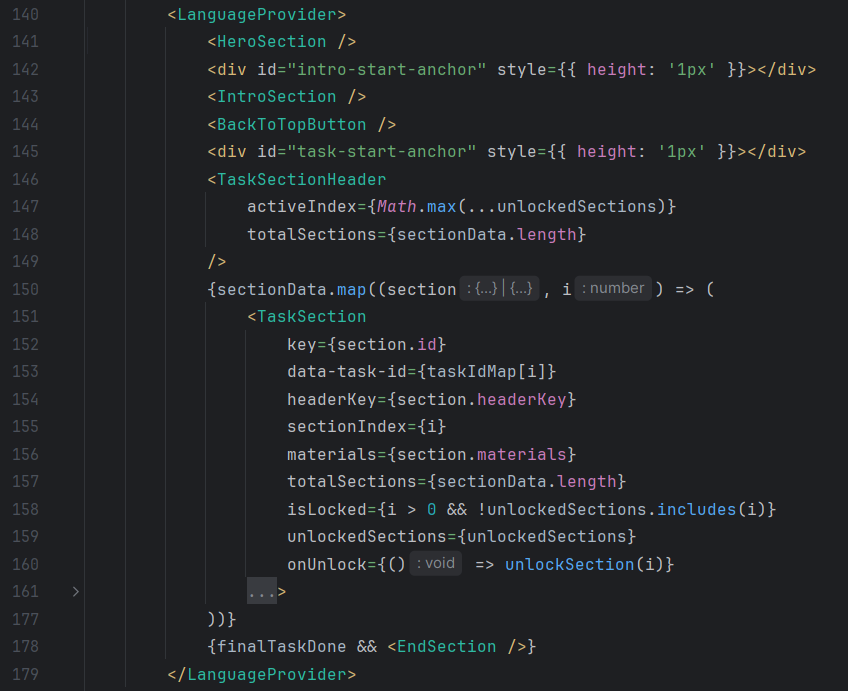
\includegraphics[width=14cm]{Media/app_composition.png}
 \caption{High-level architecture of the website's code components}
 \label{fig:app_composition}
 {\raggedright \small{Source: created by the author, file src/App.js, 2025}\par}
\end{figure}

\subsubsection{Introductory Section}
The hero landing area is designed to give the visitor a very quick impression of the website being related to their recognition through Open Badges, with some visual flair, therefore, it has a bright, deep blue background. 
Some of the basic elements other than headers are a localisation switch between English and Lithuanian, as well as an "About Us" section. 
Due to it being relatively lightweight, it has been developed as a slide-out to reduce clutter as well as maintain the one-page technical requirement. 
Notably the intention within the hero area is to get the user to begin with their progression as quickly as possible. 
A timer is running upon landing within the website that displays a "staircase" of keywords such as "Metadata", "Proof", "Value" and "Skill". 
This guides the user's attention down the page, where a pulse animation plays on the "Start" button, ideally causing the user to begin their journey. 
Upon clicking, the user is scrolled to a display of the introductory section, which is concerned with telling the user only the very core facts about the website:

\begin{itemize}
    \item What is the goal of this website?
    \item How to succeed?
    \item Explanation of how points work.
    \item Core progress tracking information.
\end{itemize}

To better maintain the user's attention, a scroll-linked \acrshort{svg} path follows the user along the existing <div> blocks, signifying the user's progress through the introduction. 
The section is capped off with another \acrshort{cta} button to align the user for the first task.

\subsubsection{Task Section}

To simplify development and maintain consistency and clean code principles and separation of concerns across tasks, each individual task component only implements the interaction logic and content-specific functionality. 
The remaining UI and elements are deferred to the parent TaskSection component. 
As demonstrated in Figure \ref{fig:task_layout}, a typical task component only renders localised instructional prompts, the interactive task UI (e.g., swiper, drag/drop area) as well as a conditional "Continue" button and score bubble. 
The task component is passed props like onUnlock from TaskSection, which allows it to notify the parent when the task has been completed.
The task component also has access to translated strings, session score handling, and internal states such as completed, locked, and selected answers, but these are contained within the component's internal logic.
This architecture makes it easy to expand the system. 
Any new task needs only to adhere to its own specific task content, call onUnlock() when done, and include localised prompts or completion messages. 
Each task is individually fed with a custom order and amount of text headlines and paragraphs to function as the "Materials" of the task, that is then dynamically formatted based on each task.
As a result, each task remains pedagogically distinct yet structurally consistent, ensuring a unified learning experience while supporting varied forms of gamified interaction.

\begin{figure}[hbtp]
\centering
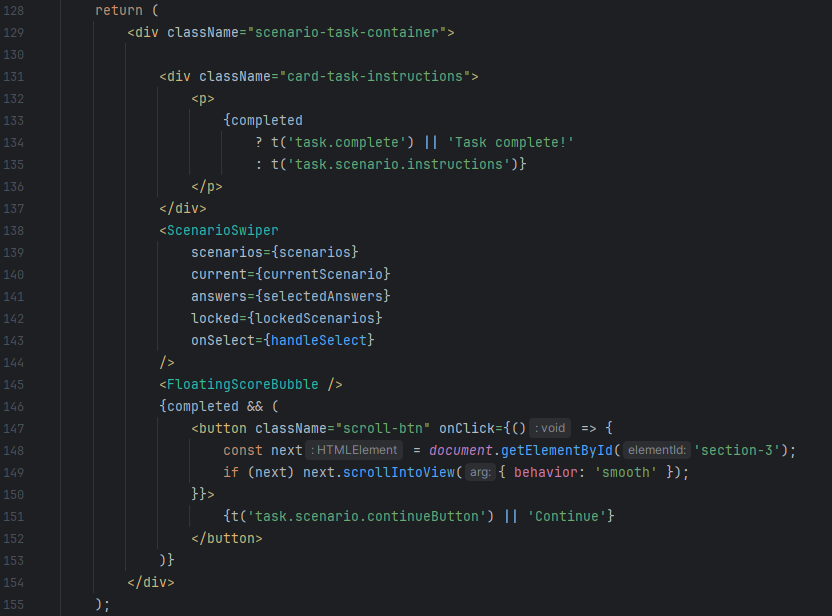
\includegraphics[width=0.8\textwidth]{Media/task_layout.png}
\caption{Code structure of the Scenario task component.}
\label{fig:task_layout}
{\raggedright \small{Source: created by the author, file src/tasks/slidingTask.js, 2025}\par}
\end{figure}

The website implements a browser-based, lightweight system for progress tracking, scoring, and user behaviour logging. 
This approach allows for responsive interactivity while avoiding the need for server-side user accounts, keeping the experience more private and fast.

\textbf{Other modular functionality on the website}:
\begin{itemize}
    \item \textbf{Local storage and progress tracking}: The website tracks user preferences and progress within the local storage of the browser that persists throughout reloads. 
    The preferences specifically track the language selected at the start and if adjusted, will always load the respective language saved.
    Each task section completion is tracked individually through local state as well.
    When a task is completed, a save function is called which adds a statement to the local storage in \acrshort{json} format with a respective identifier, e.g. taskCompletion: \{"task.card-sort":true\}. 
    Should the user reload the website, the task will autocomplete, without tampering with the user's original score.
    This information is then referenced using isTaskCompleted() function to conditionally unlock future sections in the learning path, maintaining the progression model. 
    As mentioned the user's score is also consistently tracked and updated within local storage upon completion of any section.
    Tracking the score only upon completion allows for avoiding score recalculation if the user restarts any section by reloading. 
    This storage solution is ideal for a consistent, clean and private experience, as no actual user PII \footnote{Personally Identifiable Information} is retained.
    \item \textbf{Score system}: The score system operates entirely on the frontend, with a central live score variable that syncs to both persistent storage and UI elements at specific moments. 
    The user’s current score is displayed dynamically and updated in real-time using a custom hook, useLiveScore(), which polls the live score value at the top of the screen throughout the task section. 
    Visual feedback for user actions, such as gaining or losing points upon selecting a correct or incorrect answer respectively is provided via useFloatingScore(). 
    That function triggers a dynamic function element which briefly displays the score delta using a styled floating element near the top of the screen, just below the total live score. 
    The element is either in deep blue to associate with correctness and progress, or red to indicate a mistake.
    The positioning allows the user to associate the score delta with the total score. 
    This feedback is implemented to enhance engagement and give learners further immediate confirmation of their choices.
    The score adjustments are called via adjustScore() function, which then triggers any and all necessary events as seen in Figure \ref{fig:score_update}.
    The user's total score is saved locally upon each task completion and after claiming the Open Badge is attached to the badge issuing request as a criteria addendum, to be discussed later.
    
\begin{figure}[hbtp]
\centering
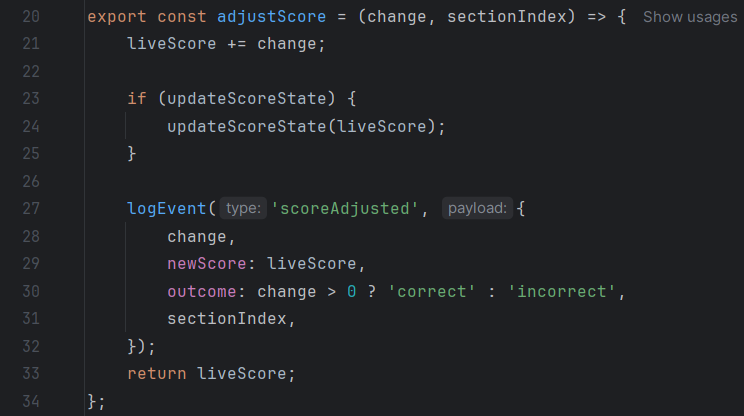
\includegraphics[width=0.8\textwidth]{Media/score_update.png}
\caption{adjustScore() function used to update user score and log outcomes}
\label{fig:score_update}
{\raggedright \small{Source: created by the author, file src/utils/scoreUtils.js, 2025}\par}
\end{figure}

    \item \textbf{Logging of the user's experience}: The system logs significant user interactions via a dedicated event logger module. 
    Each task unlock, score adjustment, or badge claim is recorded with a timestamp and optional payload metadata, as seen in Figure \ref{fig:logging}. 
    The log is stored in memory as a simple JavaScript array, allowing it to be serialised and submitted to the backend for future analysis. 
    This logging framework provides value for both quantitative evaluation of learning engagement later on and debugging during development. 
    These logs are collected and submitted upon submission of the badge claim form, delivering it in \acrshort{json} format to the backend.
\begin{figure}[hbtp]
\centering
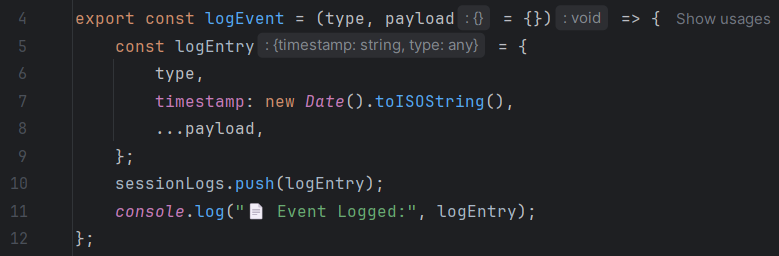
\includegraphics[width=0.8\textwidth]{Media/logging.png}
\caption{logEvent() function, which is responsible for appropriate formatting and creation of each significant interaction log, utils/eventLogger.js, 2025}
\label{fig:logging}
\end{figure}
    \item \textbf{Task question randomisation}: The following feature has been implemented based on feedback during mid-development from supervisors. 
    To improve task replayability and reduce answer memorisation, all tasks implement a randomisation strategy. 
    As seen in Figure \ref{fig:shuffling}, each array of questions and/or their answers is reshuffled within each load, using the shuffleArray() utility function. 
    This ensures that the item order is unpredictable between sessions. 
    For example, the scenario task will present the scenarios in random order, with the answers randomly rearranged, or the metadata task will display a randomly rearranged list of the metadata elements.
\end{itemize}

\begin{figure}[hbtp]
\centering
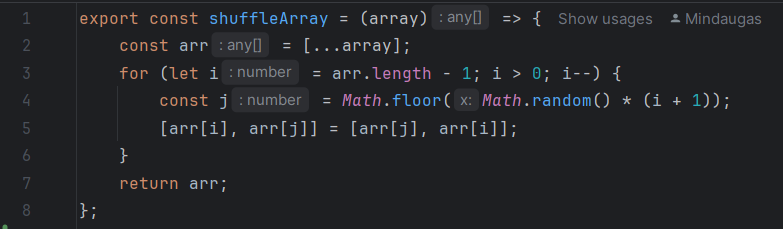
\includegraphics[width=0.8\textwidth]{Media/shuffling.png}
\caption{shuffleArray() function for randomizing answer and question order}
\label{fig:shuffling}
{\raggedright \small{Source: created by the author, file src/utils/shuffle.js, 2025}\par}
\end{figure}

The sequence of tasks was deliberately structured to progressively introduce key concepts surrounding Open Badges through interactive learning. 
Task 1 introduces the idea that badges are closely tied to specific skill recognition, particularly soft skills often overlooked in formal credentials. 
The task challenges the user to differentiate which skills the Open Badges represent. 
Task 2 is more formal and is focused on the required metadata embedded in each badge, which guarantees transparency and verifiability. 
Task 3 shifts to contextual evaluation, where users explore real-world scenarios and relevant badge issuance and reflect on the multiple competencies a single badge might represent. 
Task 4 introduces the idea of badge curation by demonstrating how individual badges can be merged into "Meta" or "Uber" badges that reflect broader or combined achievements. 
Finally, Task 5 shows Open Badges from the perspective of both students and employers, emphasising their dual value as a tool for personal development and recognition. 
This user journey of tasks builds a narrative that is meant to introduce and explain all of the core elements surrounding Open Badges.


\textbf{Task 1: Card Sorting}

The first interactive activity on the website is a card sorting task designed as a basic classification task. 
In this task, users are presented with a bank of draggable skill statements from the "Skills" field.
They must be sorted into one of two columns, labelled as "hard" and "soft" skills. 
Correct placements result in green visual confirmation, score increase and the card becoming fixed in place, while incorrect placements trigger red highlights, a deduction in points with a score deduction bubble, and a contextual explanation overlay. 
Incorrect cards remain draggable, allowing the user to correct their mistake, supporting mastery through trial and error.

The task utilizes the @dnd-kit/core library.
It's a lightweight and extensible drag-and-drop toolkit for React. 
This library was chosen for its strong support of mobile and touch devices, which is critical for a mobile-first layout. 
The main component wraps its content in a <DndContext> element, which handles drag state and event resolution across all draggable and droppable zones. 
Each card is wrapped individually in a DraggableCard component utilising useDraggable(). 
This function allows dragging of the element on both mobile and desktop devices without creating a jarring experience, such as accidentally scrolling with the card. 
Each column is then rendered through DroppableColumn, powered by useDroppable().
A drag event is resolved within the handleDragEnd() function, which determines whether the dragged card was placed into the correct column based on its intended column. 
Correct placements trigger the adjustScore() function with a positive value, and incorrect attempts deduct points and trigger the feedback modal, displaying an instructional message linked to the card’s mistakeKey. 
The card bank is randomised using the shuffleArray() utility on load, reducing memorisation of answer locations between attempts.
The task prompt styled in yellow is located between the columns and skills bank, vertically, to clearly instruct the user and draw necessary attention.
The in-progress task view can be seen in Figure \ref{fig:cardTask}.

\begin{figure}[hbtp]
\centering
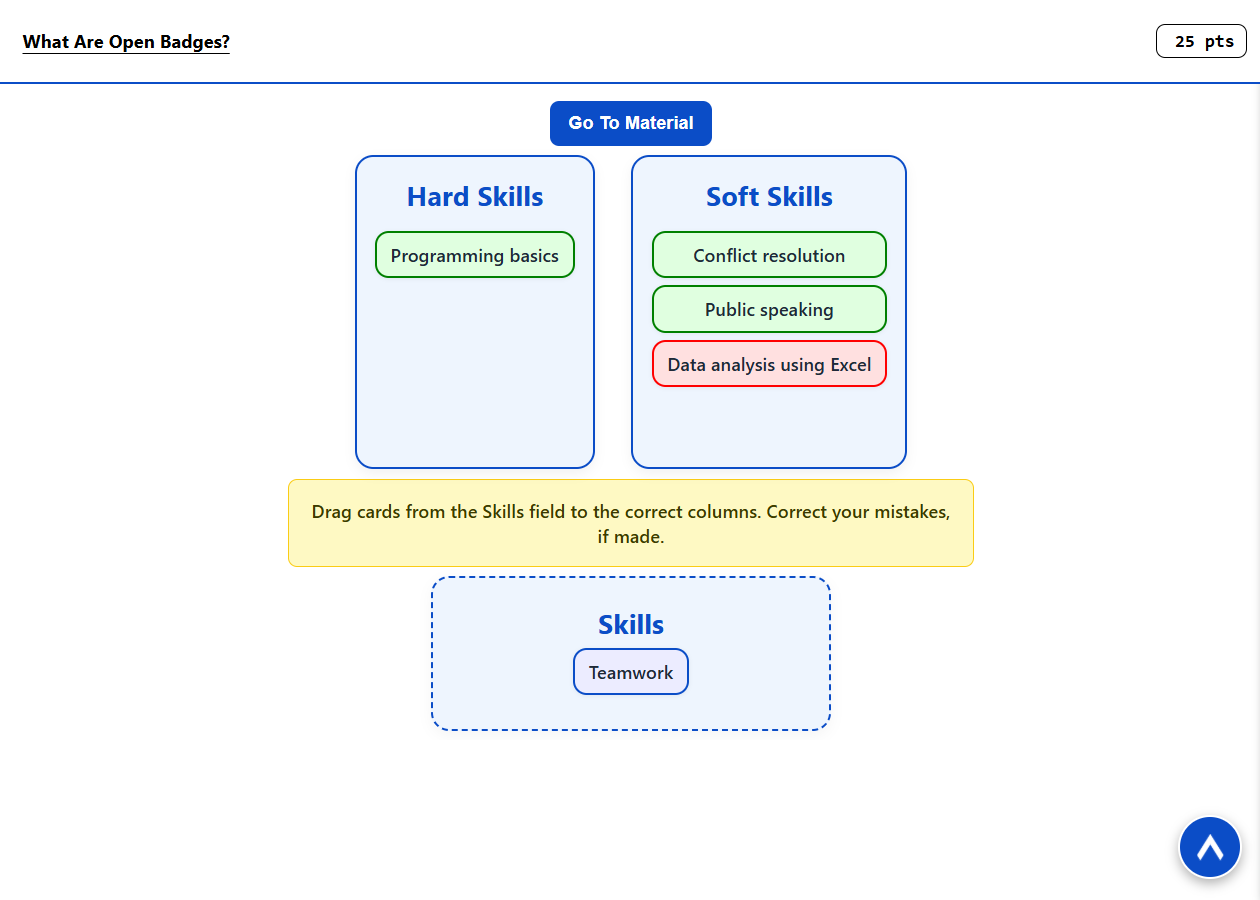
\includegraphics[width=0.8\textwidth]{Media/cards.png}
\caption{Card Sorting task in-progress}
\label{fig:cardTask}
{\raggedright \small{Source: created by the author, file src/tasks/cardTask.js}, 2025\par}
\end{figure}

Once all cards are placed correctly, the section is marked as complete, the score is persisted, the skills bank collapses and the task prompt is updated to state "Task completed!", to inform the user to continue with the next task. 
The parent TaskSection is notified via onUnlock(), allowing the next task to become accessible and the "Continue" button shows up for the user to conveniently progress.


\textbf{Task 2: Metadata Selection}

The second task introduces users to the structural components of an Open Badge by asking them to select only the necessary components of valid badge metadata. 
The goal is to reinforce understanding of which attributes are required for a badge to be considered valid and verifiable. 
Those elements are the issuer, badge earning criteria, issue date, encrypted recipient email, achievement description and badge class.

Here the task prompt is displayed at the top to be clearly visible and not interfere with the task display. 
It also appropriately updates upon completion.
This task uses a button grid for basic interactivity. 
Each enhance the simplicity of the task, each item appears as a button within a split “staircase” layout, which is displayed scaled based on the user's screen size whether on desktop or mobile.
The interaction is a set of ten shuffled elements, each mapped to either a valid metadata field or a plausible but incorrect distractor (e.g., “social media links”). 
When a user selects an option, the task validates whether it belongs to the Open Badge metadata schema. 
Correct answers trigger score gains and visually lock the button in place with a green highlight, and incorrect answers deduct points and display a feedback overlay with an explanation, using a mistakeKey.
A floating score bubble provides immediate feedback for each action as well.
An in-progress view of the task can be viewed in Figure \ref{fig:metadataTask}.

\begin{figure}[hbtp]
\centering
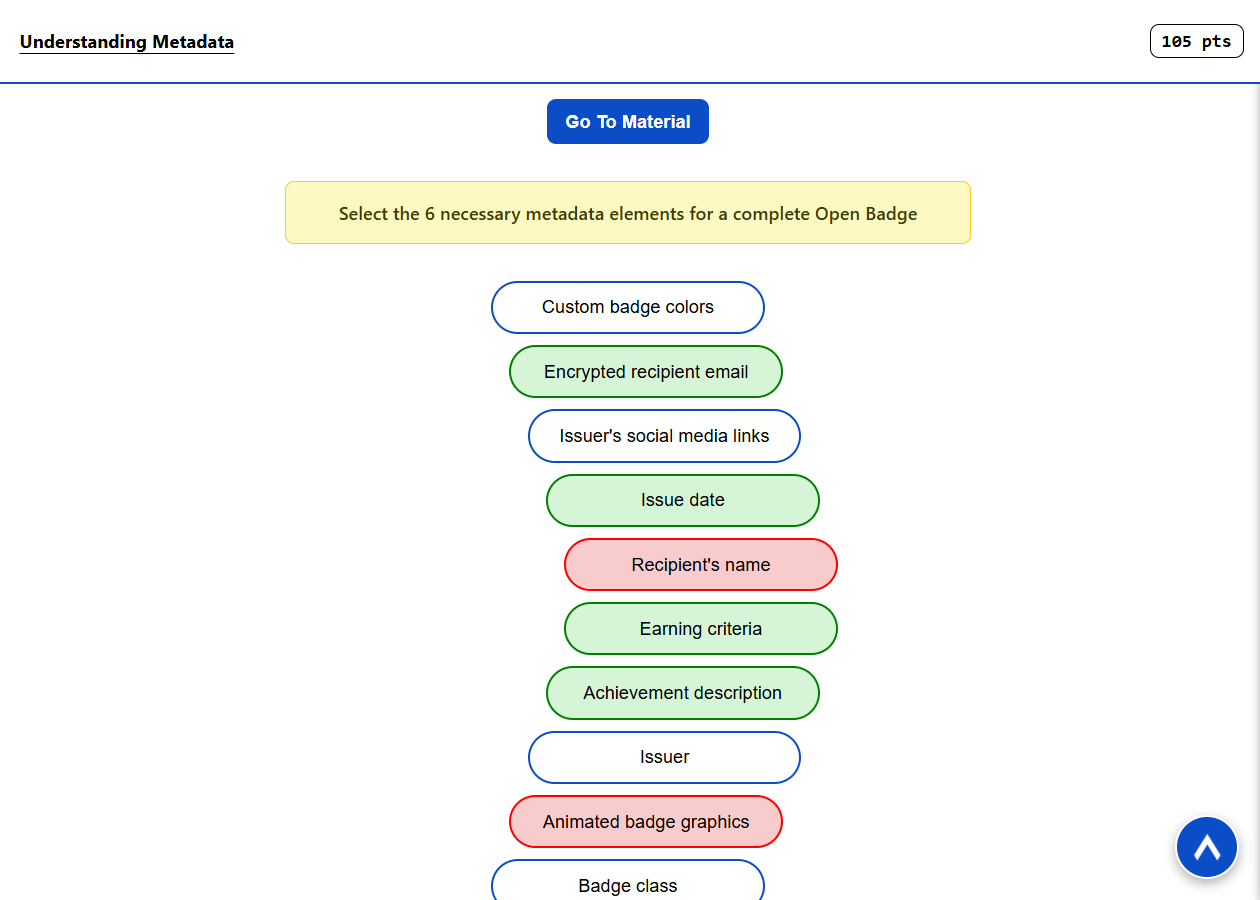
\includegraphics[width=0.8\textwidth]{Media/metadata.png}
\caption{Metadata Selection task in-progress}
\label{fig:metadataTask}
{\raggedright \small{Source: created by the author, file src/tasks/metadataTask.js}, 2025\par}
\end{figure}

The task uses internal state to track each selection (selected), and completion is detected once all correct elements have been chosen. 
As with other tasks, the system records progress using saveTaskCompletion(), locks the interface, and calls onUnlock() to reveal the next section.
Completion also triggers the "Continue" button to appear directly under the task, which would scroll down and realign the user at the next task.

 
\textbf{Task 3: Scenario-Based Selection}

The third task introduces contextual reasoning by asking users to select the most appropriate Open Badge for a given real-world scenario. 
It aims to deepen understanding of how badges represent specific competencies and apply to practical achievements. 
Each scenario presents a short narrative, followed by three visually distinct badge options, only one of which correctly reflects the competencies demonstrated in the story.
In retrospect, the received feedback pointed to this task being confusing to the user due to certain wording present within the scenarios, which caused mild frustration for a small number of users. 
After investigation, it was found that there were both a localization issue and a wording issue which was causing the frustration.
That leads to the conclusion that exact wording and maintenance of localisation are very important for an enjoyable experience.

The scenario logic is separated into a helper component, ScenarioSwiper.jsx, which manages animated transitions between scenarios using Framer Motion's <AnimatePresence> and <motion.div>. 
Only one scenario is rendered at a time, reducing distraction and allowing for focused attention. 
The swiper detects the current scenario via ID and animates horizontal transitions as users progress(select correct answers), simulating a card-swiping interface. 
Each badge option is rendered as a clickable button containing both text and an image of the corresponding badge. 
Like in previous tasks, selecting correct and incorrect answers will trigger the element to change colour and display a score delta, respectively. 
Each answer is locked after selection, so the user would not accidentally reduce their points, as the task does not progress until the correct answer, specifically, is selected.
Each scenario and possible answers are shuffled arrays to vary the orders across sessions. 
The in-progress view of the task can be seen in Figure \ref{fig:scenarioTask}. 
Once all three scenarios are answered correctly, the saveTaskCompletion() and onUnlock() functions are triggered, updating the task prompt and revealing the "Continue" button, as well as revealing the next section.

\begin{figure}[hbtp]
\centering
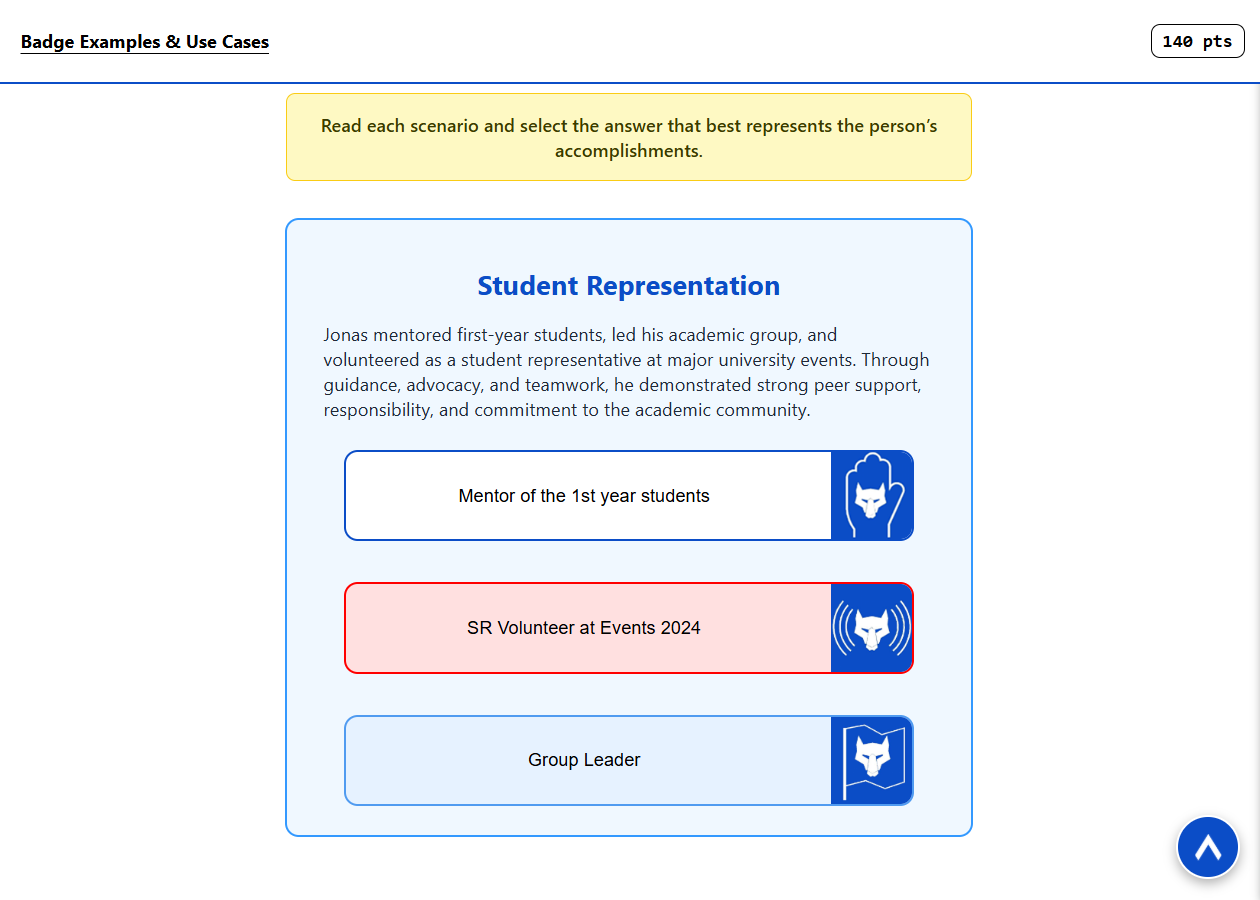
\includegraphics[width=0.8\textwidth]{Media/scenario.png}
\caption{Scenario-Based Selection task in-progress}
\label{fig:scenarioTask}
{\raggedright \small{Source: created by the author, file src/tasks/scenarioTask.js}, 2025\par}
\end{figure}


\textbf{Task 4: Badge Merging}

This task simulates the combination of smaller competence badges into a larger Meta badge. 
The user must drag smaller badge elements into a central slot, triggering a visual merge animation. 
The task builds on a key feature in badge ecosystems where multiple smaller achievements are combined into a badges of a new class, such as the "Meta" badge.
Notably, this task contains no possibility for incorrect answers, as such no mistake feedback is necessary.
This task is meant to function as a time for the user to relax, enjoy the animations and visual effects, and continue to the next and final task relatively quickly. 

In this task, users are presented with three smaller badges, a central merge zone (yellow circle, the \acrshort{cta} colour), as well as a task prompt instructing to drag the badges into the circle.
Using the @dnd-kit/core library again, learners are able to drag badges into the central drop area. 
The user interaction is handled through the DndContext, with each badge wrapped in a DraggableBadge component and the central area implemented as a DropZone. 
Internal state tracks which badges have already been placed and triggers a score reward via adjustScore() on each valid drop. 
Once all required badges are dropped, the task is marked complete, and a delayed animation video unlocks the next section after approximately seven seconds, allowing the user time to view the merge effect animation.
The animation that plays in question is a previous coursework project created with the intention of being used for this project specifically. 
It is a complex vector animation compiled as .MP4 file, that uses pre-loading as soon as the landing page is loaded for the user. 
The video is approximately 8 seconds long and is of approximately 700 KB in size, without loss in quality due to relatively simple vector graphics compression. 
A frame of the animation playing can be seen in Figure \ref{fig:mergeTask}, (b).

This task is supported by a helper component, MergeCenterDisplay, which handles dynamic text and visual content inside the merge zone based on drop progress. 
To represent the user's progress visually, the task uses a custom 
ProgressRing component. 
The ProgressRing component is called inside of MergeCenterDisplay. 
It is a React \acrshort{svg} that simply renders two circles, one of which is a static background circle, and the other one is a dynamic, green foreground circle, that is filled in based on user's progress, with a simple formula:
\progresscalc{current}{total}
Once dropped, each badge contributes to a looping animation that has the dropped badge icon orbiting within the inner area of the progress circle, on a select trajectory based on drop order, which can be seen in Figure \ref{fig:mergeTask} (a), simulating badge accumulation. 

\begin{figure}[H]
  \centering
  \begin{subfigure}[]{0.4\textwidth}
    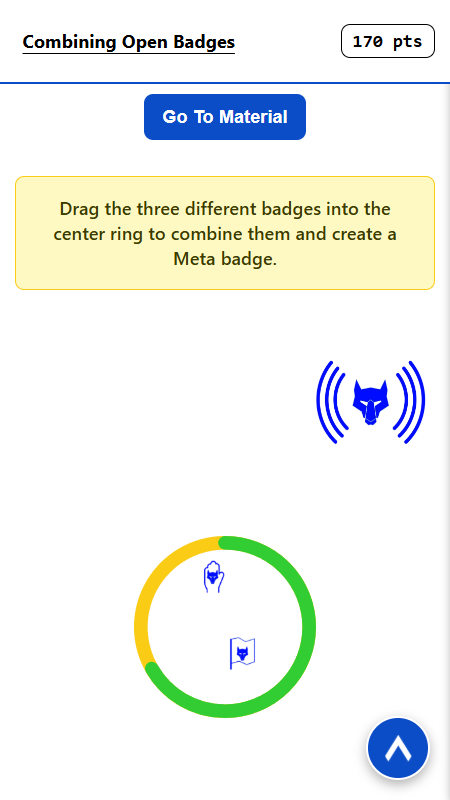
\includegraphics[width=\textwidth]{Media/merge1.png}
    \caption{Badge Merging in-progress}
  \end{subfigure}
  \hfill
  \begin{subfigure}[]{0.4\textwidth}
    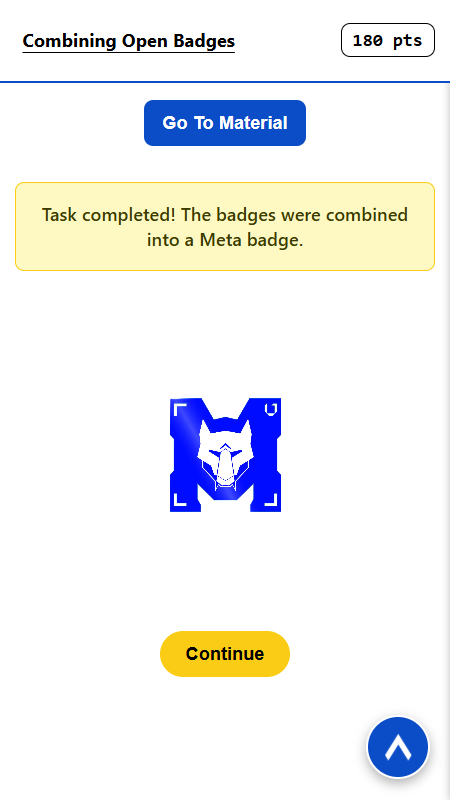
\includegraphics[width=\textwidth]{Media/merge2.png}
    \caption{Badge Merging post-completion animation playing}
  \end{subfigure}
  \caption{Badge Merging task, mobile view}
  \label{fig:mergeTask}
  {\raggedright \small{Source: created by the author, file src/tasks/mergeTask.js}, 2025\par}
\end{figure}


\textbf{Task 5: Card Classification}

The final task presents a sequence of statement cards related to the value and impact of Open Badges. 
Each card must be classified as either student-oriented or employer-oriented, reinforcing the dual value that Open Badges hold for both audiences. 
This final challenge ties together the learner’s understanding of badge value, communication and contextual application. 
The task is presented as a vertically stacked swiper or slider, where each card appears one at a time and offers two selectable categories ("Student", "Employer"). 
Correct classifications are locked in and trigger score feedback, and progress to the next card, while incorrect classifications trigger negative score feedback, providing visual guidance without penalising user flow. 
This leads to careful consideration without harsh interruption. 
The task in-progress can be viewed in Figure \ref{fig:swiperTask}.

\begin{figure}[hbtp]
\centering
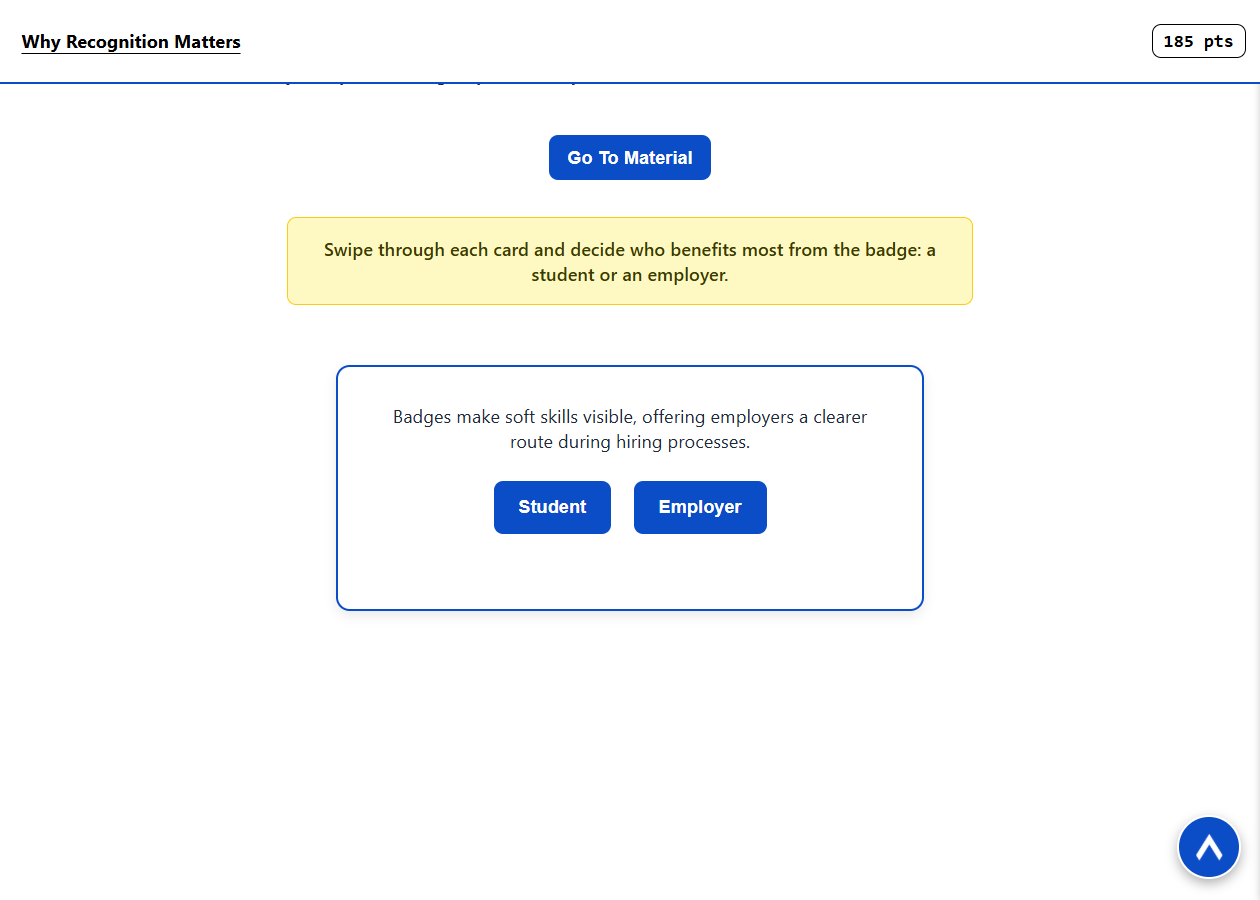
\includegraphics[width=0.8\textwidth]{Media/swiper.png}
\caption{Card Classification task}
\label{fig:swiperTask}
{\raggedright \small{Source: created by the author, file src/tasks/slidingTask.js}, 2025\par}
\end{figure}

Internally, each card's classification logic compares the selected category with a pre-defined key, which is either 0 or 1. 
The card slider is implemented using a dedicated helper component, slidingTaskHelper, which renders the current card, its classification options, and handles animations. 
It is very similar in structure to the scenarioSwiper but handles the elements differently. 
All correct classifications must be made to complete the task. 
Once completed, the task is locked, progress is stored, and the final "Finish" button appears to guide the user toward the badge issuance section. 
As with other tasks, all cards are shuffled on load using the shuffling function, to increase replayability. 

\subsubsection{End Section}

The final part of the website is only rendered upon completion of all tasks. 
This is tracked through local storage updates, checking for the task completion variable to include each section.
The section displays a basic form for the user's full name and email. 
The form utilises standard checks to ensure the user enters correct and viable information.
The submission button can only be triggered if the entered information is viable, which calls the backend with a request to issue an Open Badge for the user. 
The rest of this functionality is handled by the backend. 
The form gets replaced by the appropriate backend response based on the code returned, e.g. code 200 would lead to a success message or 500 would display an internal error message.
The end section additionally includes a "Play Again" button, which is a hold button, so the user wouldn't accidentally click it. 
After holding for a few seconds, the button scrolls the user to the top of the website while fading everything to white. 
Once the website is faded out, it wipes the user's accumulated total score and saved completed sections, then reloads the website so the tasks get reshuffled for a refreshed experience.

Together, these frontend technologies and design decisions form a responsive, gamified educational platform that adapts to user behaviour and supports pedagogical goals. By combining React’s modular strengths with carefully crafted gamified mechanics, the website delivers a rich and engaging learning experience across mobile and desktop devices.

\subsection{Backend Integration and Badge Issuance}

The backend of the gamified educational website was developed as an Express application using Node.js and deployed on Render.com platform as a lightweight, stateless \acrshort{api}. 
Its primary role is to securely manage and issue digital badges via the Open Badge Factory (from here - OBF) \acrshort{api}, while also supporting task verification and interaction logging. 
The backend architecture is purposefully minimal to preserve user privacy and reduce infrastructure complexity, with all sensitive operations encapsulated within server logic.

\subsubsection{Badge Issuance via Open Badge Factory API}

It was crucial to provide users with viable, verifiable and trusted Open Badges upon website completion. 
Due to technical limitations, it was not possible as of the time of writing this to integrate with the Vilnius Tech system on badgecraft.eu, so instead an alternative was chosen in Open Badge Factory. 
They utilise a Mozilla Open Badge standard for issuance, secured by OAuth-2, and allow for badge issuance automation via their \acrshort{api}, which is a perfect fit for the project. 
Upon form submission on the frontend, the frontend dispatches POST request containing the user’s email, name, final score, and language preference. 
This triggers a secure server-side sequence:

\begin{enumerate}
\item \textbf{Access Token Retrieval}: The backend authenticates itself by sending the preconfigured client\_id and client\_secret to OBF’s token endpoint at \textit{/client/oauth2/token} in an encoded format for security reasons. The full code of this retrieval can be seen in Figure \ref{fig:get_token}. 
If successful, a temporary OAuth-2 access token is returned. 
\begin{figure}[hbtp]
\centering
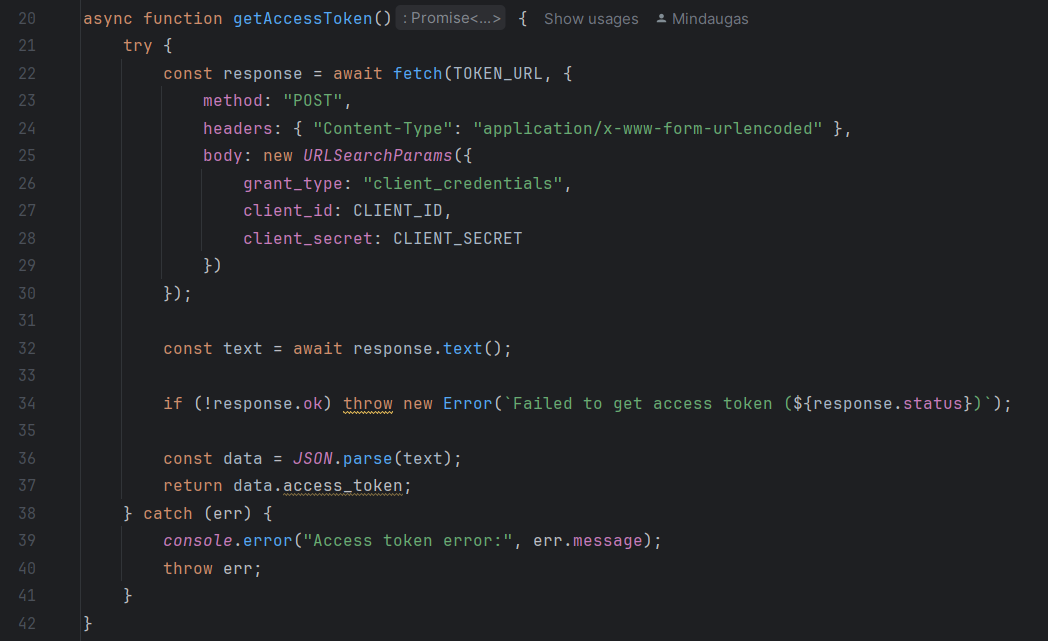
\includegraphics[width=0.8\textwidth]{Media/get_token.png}
\caption{Access Token retrieval backend function}
\label{fig:get_token}
{\raggedright \small{Source: created by the author, file backend/server.js, 2025}\par}
\end{figure}
\item \textbf{Existing Badge Check}: With the token, the server constructs and submits a GET request to OBF’s \textit{/client/client\_id/?email} endpoint. 
This returns a payload that includes issued badges and emails. 
The payload is then checked for a match within the payload and the user's submitted email. 
If a badge is already issued with the user's email, the error code of 409 is returned and a relevant message is delivered to the user on the frontend. 
Giving out multiple copies of the same badge, or even endlessly updating the badge would degrate the value of Open Badges. 
\item \textbf{Badge Issuance Request}: If the existing badge check gets passed, a new payload is created. 
It includes the access token, the user's name, email, submission date and individualised criteria addendum (updated with the user's final score) and a localised congratulations email(based on user's preference saved in local storage). 
Notably, additionally specified is the \textit{api\_consumer\_id = "standalone"}, which was not specified by the \acrshort{api} documentation as a necessary element to include, but in fact would consistently fail the issuance if excluded. 
This was discovered through extensive and thorough debugging. 
Its inclusion can be seen within the badge issuance payload in Figure \ref{fig:payload} and caused multiple setbacks during backend development.
The payload is then submitted as a POST request to \textit{/event/client\_id/badge\_id/issue}.
\item \textbf{Result Processing}: The backend verifies the response from OBF, logs the result internally, and returns a success or error message to the frontend. 
If the badge has already been issued for the user’s email, the backend returns a 409 status, preventing duplicates, a 200 status if the badge is successfully issued, or a 500 status for general errors.
\end{enumerate}
\begin{figure}[hbtp]
\centering
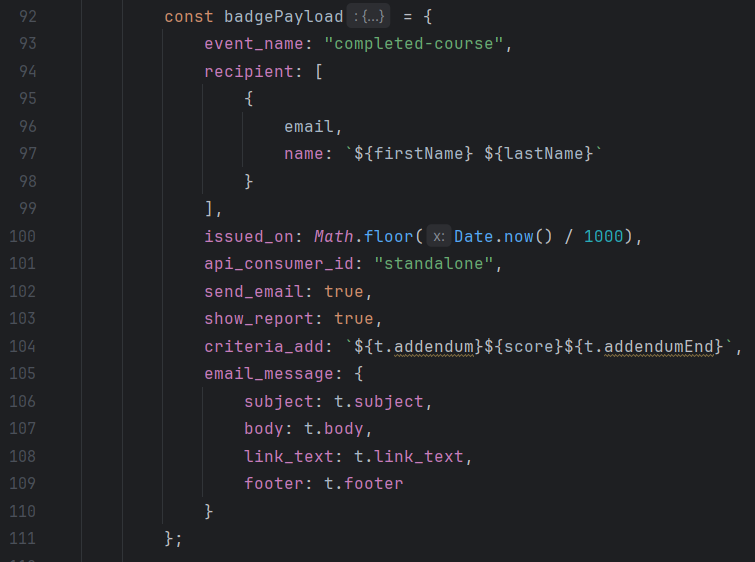
\includegraphics[width=0.8\textwidth]{Media/payload.png}
\caption{Badge issuance payload setup}
\label{fig:payload}
{\raggedright \small{Source: created by the author, file backend/server.js}, 2025\par}
\end{figure}
The client secrets are handled exclusively within the backend environment. 
This architecture ensures that no sensitive client secrets are ever exposed to the browser, because if it were handled via frontend, which is also possible, React framework would expose all environment variables. 
All credentialed communication with the Open Badge Factory occurs strictly server-side, maintaining full compliance with security best practices. 
The badge response is formatted in \acrshort{json} and parsed before returning a confirmation message to the user-facing application.

\subsubsection{Session Logging and Progress Tracking}

To support analytics and debugging without requiring user authentication, the website implements session-based logging. 
On first load, a unique session identifier is generated on the frontend and stored in local storage. 
This session ID is attached as the header to all of the log messages and progress data that will eventually get sent to the backend.
As previously discussed, each significant event, such as score adjustments, task completions, or badges, is logged through a backend endpoint at \textit{/api/log} that receives structured \acrshort{json} payloads. These logs are:

\begin{itemize}
\item Persisted as individual session files in the directory.
\item Indexed by session ID for traceability and analysis.
\item Accessible via a read-only interface for development and analysis review.
\end{itemize}

This setup allows the system to track meaningful interactions while avoiding the storage of personally identifiable information (PII), maintaining both privacy and transparency. 
Notably, during testing, an issue occurred where the backend server would come down for maintenance, and the storage solution did not prove to be persistent. 
Luckily, the terminal was persistently tracking submission, and all relevant data were successfully recovered. 
For a future reimplementation with Vilnius Tech, this would have to be reviewed based on the technology available. 
A sample log includes fields such as:

\begin{itemize}
\item Unique session identifier.
\item Total user score at submission.
\item UTC timestamp for badge issuance event (if applicable).
\item A counter of correct and incorrect answers.
\item Array of event objects, each containing event type, timestamp, and metadata for score changes.
\end{itemize}

\subsubsection{API Design and Structure}

The backend exposes a set of endpoints summarised as follows:
\begin{itemize}
\item Badge issuance via OBF’s \acrshort{api} with the endpoint \textit{/api/issue-obf-badge}.
\item Accepts structured interaction logs from the frontend and saves them to the backend upon completion at \textit{/api/log}.
\item Retrieves a single session’s full event log for testing and analysis purposes at \textit{/api/logs/:sessionId}.
\item Lists summaries of all stored sessions for basic analytics at \textit{/api/sessions}.
\end{itemize}
No personal user data is collected unless voluntarily provided for badge issuance (e.g., email), which is stored transiently and passed directly to the OBF API. 

\subsection{Technical Limitations}

While the system successfully delivers an engaging and functional gamified learning experience, a number of technical limitations were encountered during implementation that shaped design decisions and constrained the project.

First, the backend operates without persistent user accounts or authentication mechanisms and the free or cheap(there was a necessary switch during development) hosting service utilised for the project has caused both consistency and persistence issues. 
Therefore, all information is saved locally until it is delivered to the server, where currently some of the data has to be checked and stored elsewhere manually in case of the hosting service's forced redeployment of the backend. 
While the backend is lightweight, private for the end-user, fast and functional, it introduces a certain degree of fragility which should be considered upon final integration into a system. 
Additionally, currently, badge reissuance is not possible without administrative intervention or additional verification.

Second, although initial plans considered integrating with Vilnius Tech’s internal badge infrastructure, the decision was made to issue Open Badges via the external Open Badge Factory (OBF) API. 
This change was due to technical and institutional constraints, including a lack of public badge-issuing endpoints on badgecraft.eu (the system provider for Vilnius Tech) and limited documentation within the university system. OBF provided a reliable and standards-compliant alternative, albeit with its own integration challenges. 
The \acrshort{api} access on OBF is also exclusive to a paid service. 
For development purposes, an extensive trial was available to create a proof-of-concept. 
In the future, however, badge delivery is expected to be unavailable, unless the change to badgecraft.eu is completed.

Third, the badge claiming process relies on user-provided data, submitted through a frontend form. 
Although basic validation is applied, there is no real-time email verification or confirmation step, which opens the possibility of incorrect or unverified badge claims. 
Additionally, it is difficult to verify the person who claimed the actual badge without more tools. Future implementations could mitigate this by integrating optional email confirmation using institutional SSO authentication systems, if available.

On the frontend, ensuring responsive and interactive behaviour across various screen sizes, especially for mobile-first design, required extensive custom logic. 
Scroll-triggered visual effects, such as the animated \acrshort{svg} zigzag path and section snapping behaviours, were particularly complex to tune across mobile browsers with varying scroll engines and event handling. 
Inconsistent behaviour was occasionally observed, particularly on niche phone models where an extremely narrow screen would have the text elements bleed into each other, causing the relevant and relative \acrshort{svg} elements to draw over the text.

Additionally, while interaction logs are captured via a local event logger and submitted alongside the badge claim, the absence of integrated analytics tools limits fine-grained insights into user behaviour, task completion time, and drop-off rates. 
This makes it more difficult to empirically assess which sections present challenges to learners or which features are most engaging. 
Notably, drop-off points were also not investigated within the testing section as well as they were considered out of scope, due to the small sample size.

With all of the technical limitations considered, the final product was still well received and achieved the necessitated goals to an extent that will be further discussed within the testing section.

\subsection{Practical Implementation Summary}
This section detailed the technical realisation of the gamified educational website designed to teach about and promote open badges. 
Drawing from the design principles established earlier, the implementation process translated layout logic, gamified structures, and pedagogical strategies into functional frontend and backend components. 
Key technologies were employed to ensure responsive interaction, progressive task flow, and secure badge issuance. 
The integration of a third-party API, particularly for open badge management, presented both opportunities and constraints, some of which required design compromises or future planning for institutional deployment. 
This makes it a functional final programming product that is available for user testing and evaluation.
\newpage
\newpage
\section{EVALUATION OF THE IMPLEMENTATION}

\subsection{Methodology}

To evaluate the effectiveness of the implemented educational website on Open Badges, and draw actionable conclusions for future studies and improvements to make, a structured methodology was adopted that combined quantitative performance tracking with qualitative user feedback. 
The aim was to assess not only how well users performed but also how they experienced the site’s content, structure, and gamification features. 

\subsubsection{Data Collection Sources}
The evaluation was based on two core data streams:
\begin{enumerate}
    \item \textbf{Task Interaction Data:} Each user completed five sequential interactive tasks, designed to progressively introduce the key concepts behind Open Badges. 
    Every answer and completion interaction was tracked to log the following data points:
    \begin{itemize}
        \item Correct and Incorrect answer counts.
        \item Time of each answer.
    \end{itemize}
    \item \textbf{Post-Session Survey:} After completing the tasks, users were prompted to complete a structured survey comprising 8 statements for numeric answers and a set of required and optional questions with written answers. 
    Ratings were on a 4-point Likert scale (1 = strongly disagree, 4 = strongly agree). 
    This forced users to pick a neutral stance. 
    The questions were grouped into three thematic categories:
    \begin{itemize}
        \item \textbf{Gamification}: Measured the motivational effectiveness of game-like elements.
        \item \textbf{Enjoyment}: Assessed user experience and interface satisfaction.
        \item \textbf{Understanding}: Evaluated perceived learning and badge comprehension.
    \end{itemize}
\end{enumerate}

The survey questions with numeric answers were the following:

\begin{itemize}
        \item The interactive tasks made the learning experience more engaging.
        \item The score system engaged me to learn more.
        \item Receiving a badge at the end felt like a meaningful reward.
        \item Was the website enjoyable to use overall?
        \item The website was easy to navigate and worked well on my device.
        \item I would recommend this site to someone interested in learning about Open Badges.
        \item I better understand the concept of Open Badges after completing this website.
        \item I understand what the issued badge represents and how it could be used.
\end{itemize}

Below is the list of written feedback questions that the participants also had the option to leave, which was collected to supplement quantitative findings.
\begin{itemize}
        \item Which task or activity did you find the most useful or engaging for understanding Open Badges? Why?
        \item Which task or activity was the least helpful or enjoyable? Why?
        \item Did the interactive elements ever confuse or distract you from the learning content?
        \item If you answered "Yes" in the previous question, please describe what confused or distracted you, and why.
        \item Did the progression system (unlocking sections as you go) help or hinder your learning experience?
        \item Any other comments, suggestions, or technical issues you encountered?
\end{itemize}

\subsubsection{Technical Stack and Tooling}

All data processing, analysis and visualisations were carried out using Python. 
It provides a transparent and reproducible environment for chart generation, computing statistical summaries, and running statistical tests. 
The Python technical stack includes:
\begin{itemize}
        \item Data manipulation via pandas,
        \item Plotting via matplotlib,
        \item Statistical analysis with scipy.stats.
\end{itemize}

To assess internal consistency within the survey categories, the following statistical analysis tools are used:
\begin{itemize}
        \item \textbf{Cronbach’s alpha}
        \item \textbf{Pearson's correlations}
        \item \textbf{Paired t-test}
\end{itemize}

Open-ended responses from participants were reviewed manually and grouped into common themes.

Finally, the count of participants is 10. 
Importantly, due to certain technical errors related to the backend service provider, some quantitative data was corrupted, and in turn, only 9 participants' data was used, with some tests having to reduce the total count to 7, due to missing or corrupt data.
The survey also had a small technical issue due to which 1 participant's results were incomplete, which led to the total number of survey responses being 9. 
All data remained anonymous throughout the process; therefore, it was not feasible to trace the recipients for resubmission.
The total samples are slightly under the anticipated data, therefore, all data is subject to significant bias.

\subsection{Analysis and Overview}

\subsubsection{Task-Level Performance Analysis}

The evaluation began with a breakdown of user performance across the five core tasks using summary statistics from Table \ref{tab:task_summary_vertical} and complementary visualisations.
Several patterns emerged:
\begin{itemize}
        \item Task 4 stands out with perfect accuracy (1.00) and the lowest average time (2.43s). 
        Notably, this task is made without a possibility to fail, and as such, the task is performed to expectations by all users.
        \item In contrast, Task 3 was the most challenging:
        \begin{itemize}
            \item It had the lowest accuracy (mean = 0.51),
            \item The highest average time per task (42.09s),
            \item And a notably high incorrect-to-correct ratio, as seen in the chart \ref{fig:corr_incorr}. 
            The task was unique in the way that the users were able to fail twice before discovering the correct answer, if attempted way to complete it was to guess the answer. 
            This made it the most punishing task, suggesting cognitive overload or design ambiguity that warrants a review of either instructional clarity or task mechanics. 
            This is corroborated by the written responses regarding the questions within the task being slightly too vague, which caused mild frustration to users. 
            This is further supported by Figure \ref{fig:acc}, where the task, while it has the longest average time per attempt, also holds the lowest accuracy. 
            This implies that additional time in this task did not yield better outcomes.
        \end{itemize}
        \begin{figure}[hbtp]
        \centering
        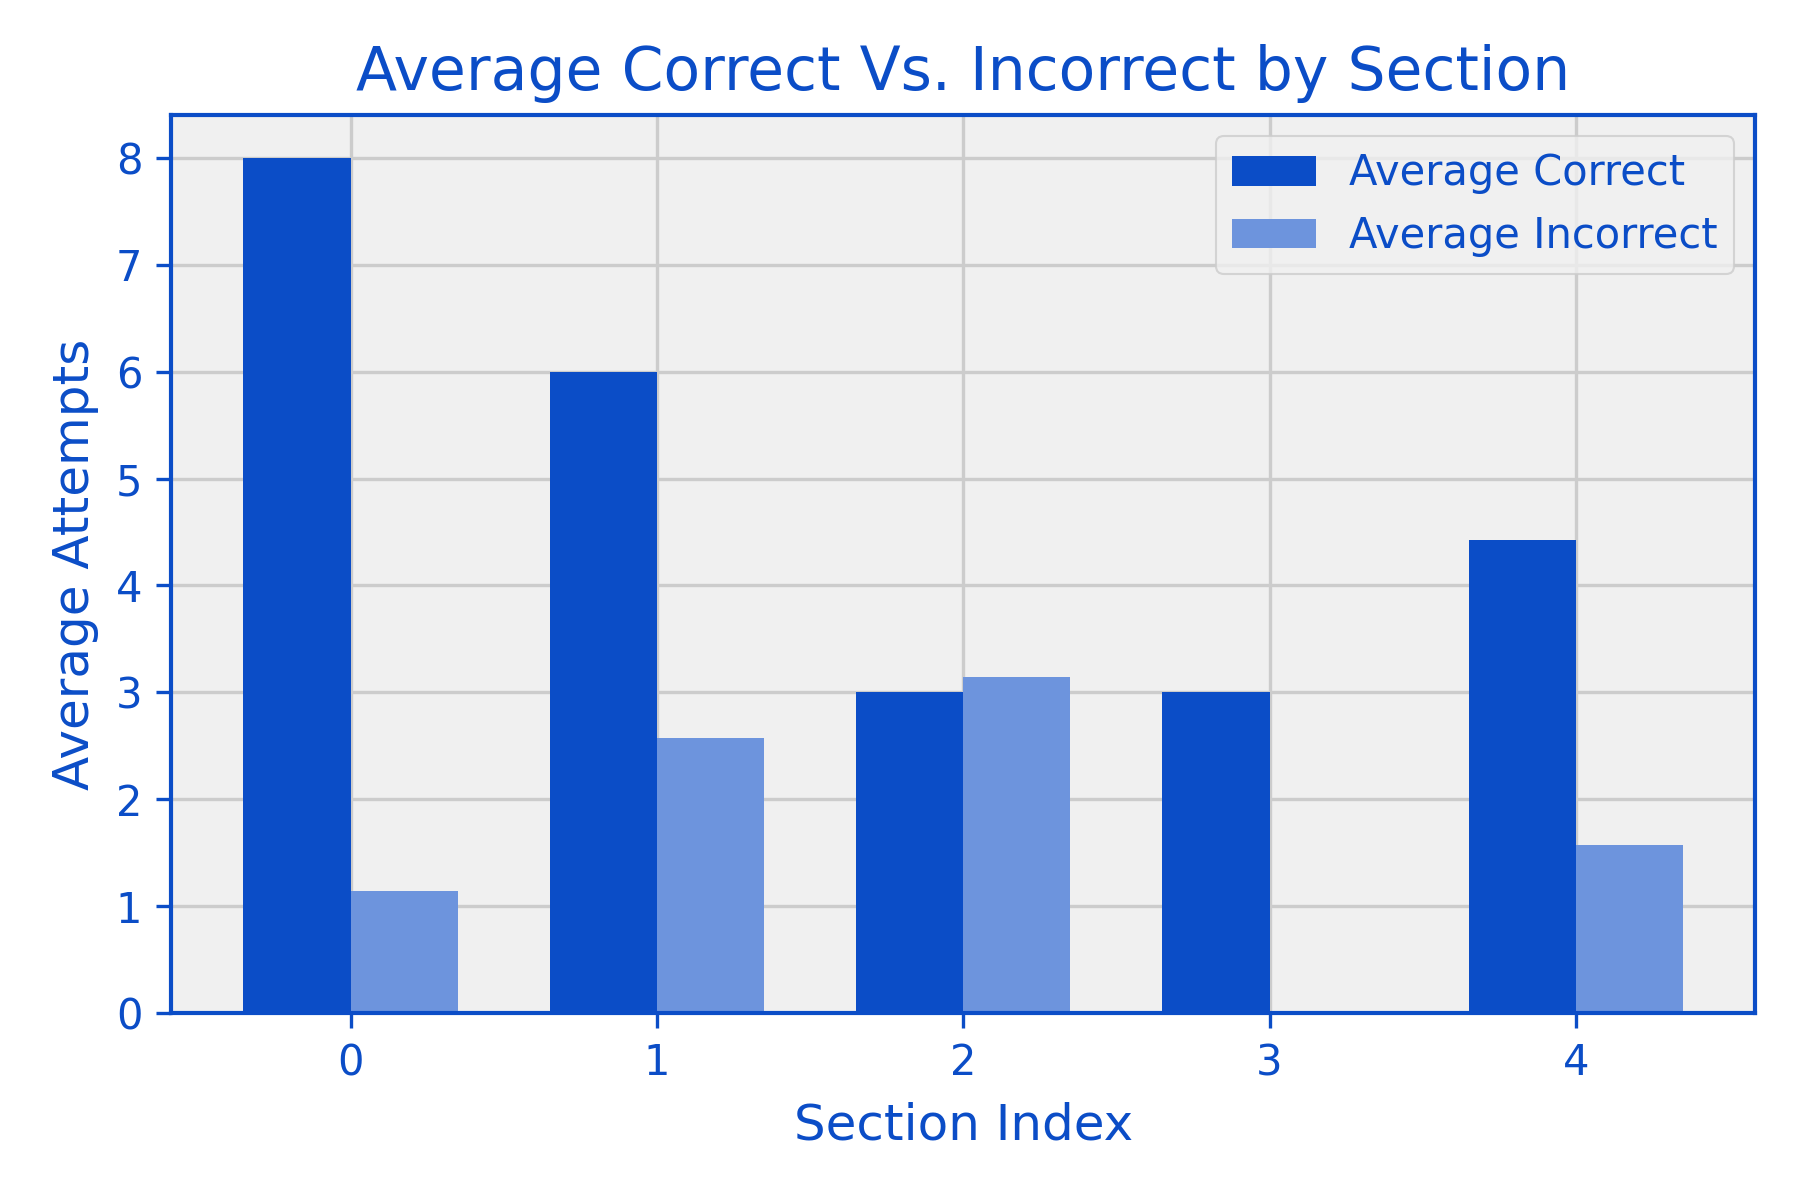
\includegraphics[width=0.8\textwidth]{figures/mean_correct_incorrect.png}
        \caption{Average Correct Vs Incorrect aggregations per task}
        \label{fig:corr_incorr}
        {\raggedright \small{Source: created by the author based on project data}\par}
        \end{figure}
        \item Tasks 1 and 2 showed intermediate difficulty, with Task 1 offering higher accuracy and slightly longer average time. 
        Task 2 showed many more incorrect attempts on average than Task 1. 
        Notably, Task 1 handles a very familiar topic to most people ("hard" and "soft" skills), in comparison to Task 2, which is about metadata. 
        \item Task 5 showed moderate difficulty but high variance, particularly in accuracy (SD = 0.17) and time (SD = 12.77s), suggesting inconsistent user experience, meaning some people found it easier than others.
        \item Overall, average time per task and accuracy display an upward trend across most tasks, as seen in Figure \ref{fig:acc}.
\end{itemize}

\begin{table}[ht]
\centering
\captionsetup{justification=raggedright, singlelinecheck=false}
\caption{Task-level summary statistics}
\begin{tabular}{lccccc}
\toprule
\textbf{Metric} & \textbf{Task 1} & \textbf{Task 2} & \textbf{Task 3} & \textbf{Task 4} & \textbf{Task 5} \\
\midrule
Avg. Incorrect     & 1.142857 & 2.571429 & 3.142857 & 0.000000 & 1.571429 \\
Avg. Total Attempts& 9.142857 & 8.571429 & 6.142857 & 3.000000 & 7.890000 \\
Avg. Accuracy      & 0.884848 & 0.719048 & 0.511735 & 1.000000 & 0.765136 \\
Std. Accuracy      & 0.098825 & 0.138253 & 0.127387 & 0.000000 & 0.168197 \\
Avg. Time (s)      & 23.556714 & 33.274714 & 42.090000 & 2.430857 & 24.135286 \\
Std. Time (s)      & 8.549135 & 29.238296 & 39.153163 & 0.981814 & 12.770451 \\
\bottomrule
\end{tabular}
\label{tab:task_summary_vertical}
\end{table}
{\raggedright \small{Source: based on results from author's implementation}\par}

\begin{figure}[hbtp]
\centering
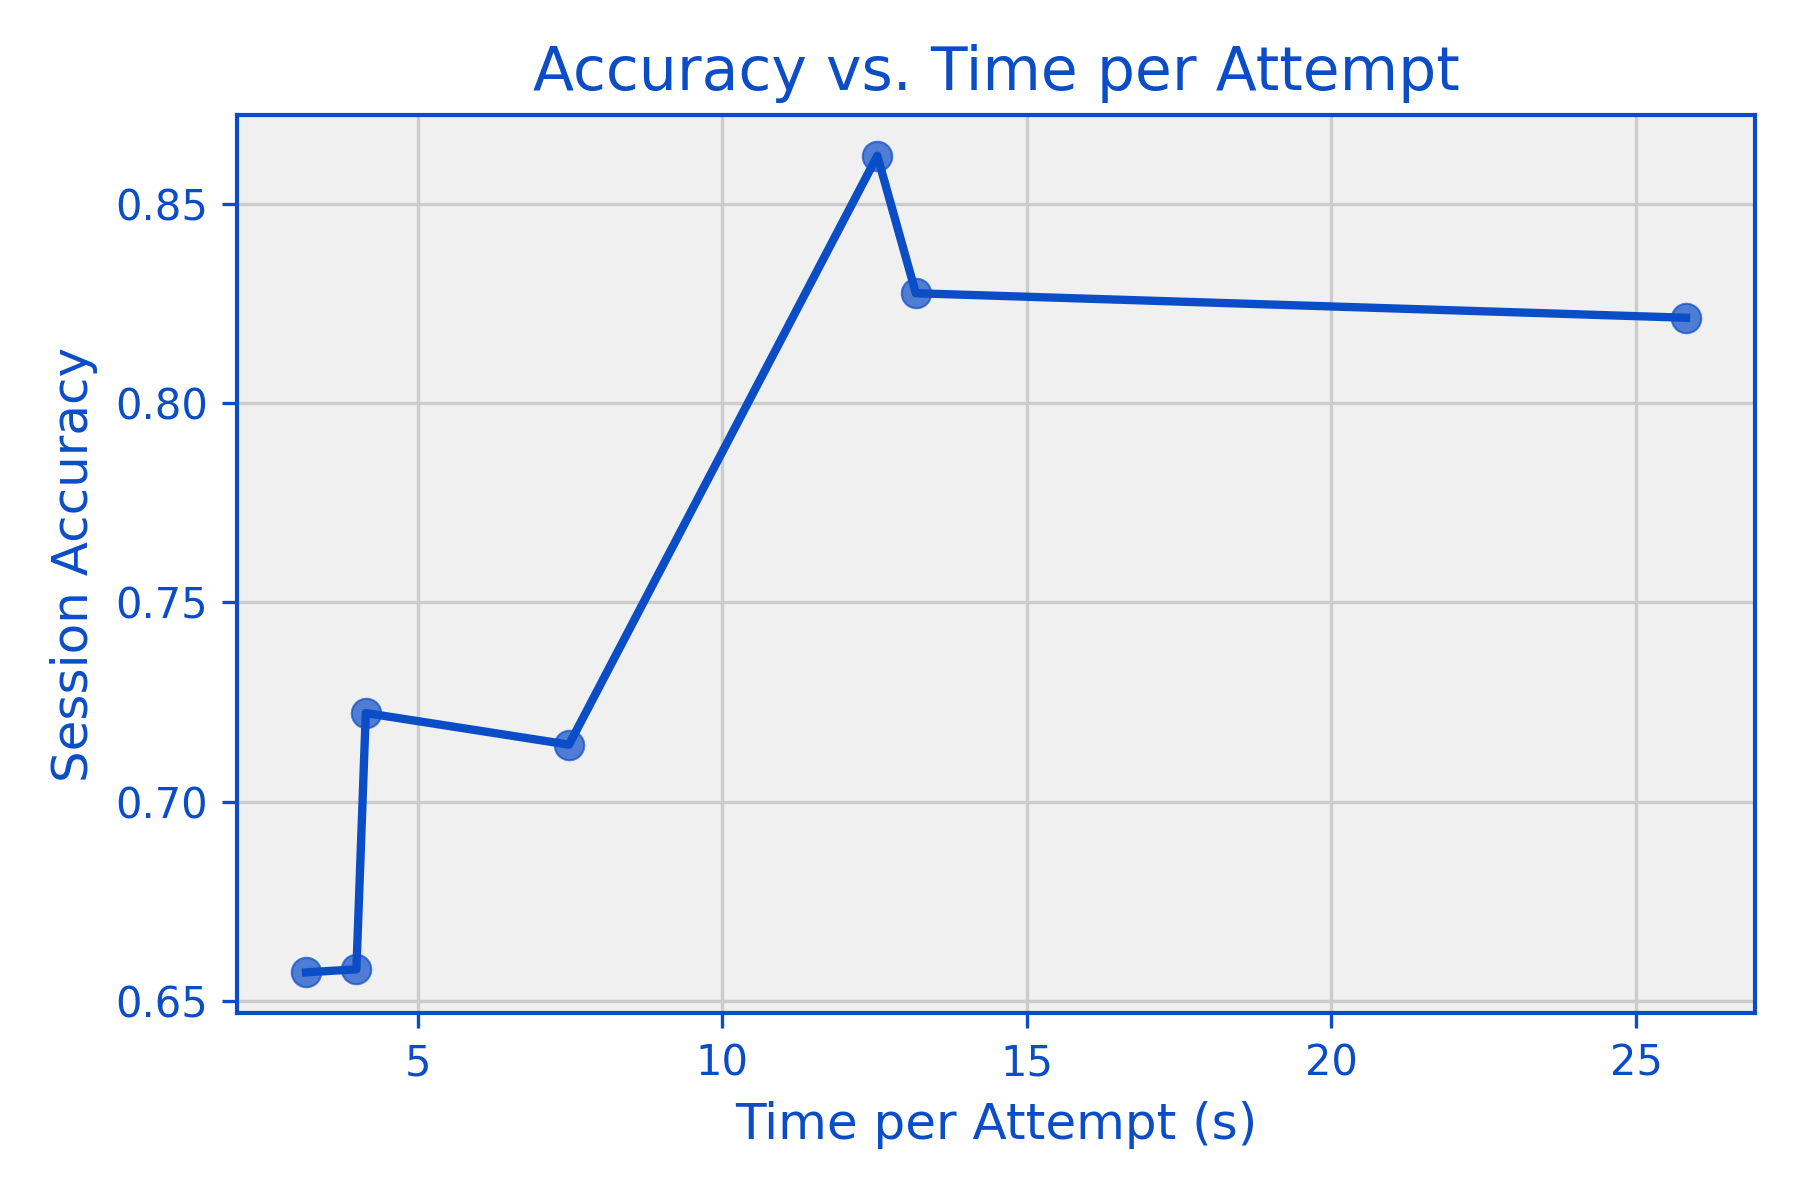
\includegraphics[width=0.8\textwidth]{figures/accuracy_vs_time.png}
\caption{Accuracy Vs Time per Attempt}
\label{fig:acc}
{\raggedright \small{Source: created by the author based on project data}\par}
\end{figure}

The heatmaps further supported these interpretations, showing clear visual hotspots in Task 3 for both extended durations and low accuracy. 
In Figure \ref{fig:acc_hm} tasks 1, 2 and 5 all have reasonable and preferable performance at 0.88 for a great starting performance, followed by a drop for increased challenge and ending with a slight recovery towards the end with Task 5.
Task 4 remains unique and Task 3 continues to stand out as a consistently failed task. 
This reinforces the need to refine its instructions, potentially implement a feedback loop, and rewrite the question prompts for the user to have improved clarity.

\begin{figure}[hbtp]
\centering
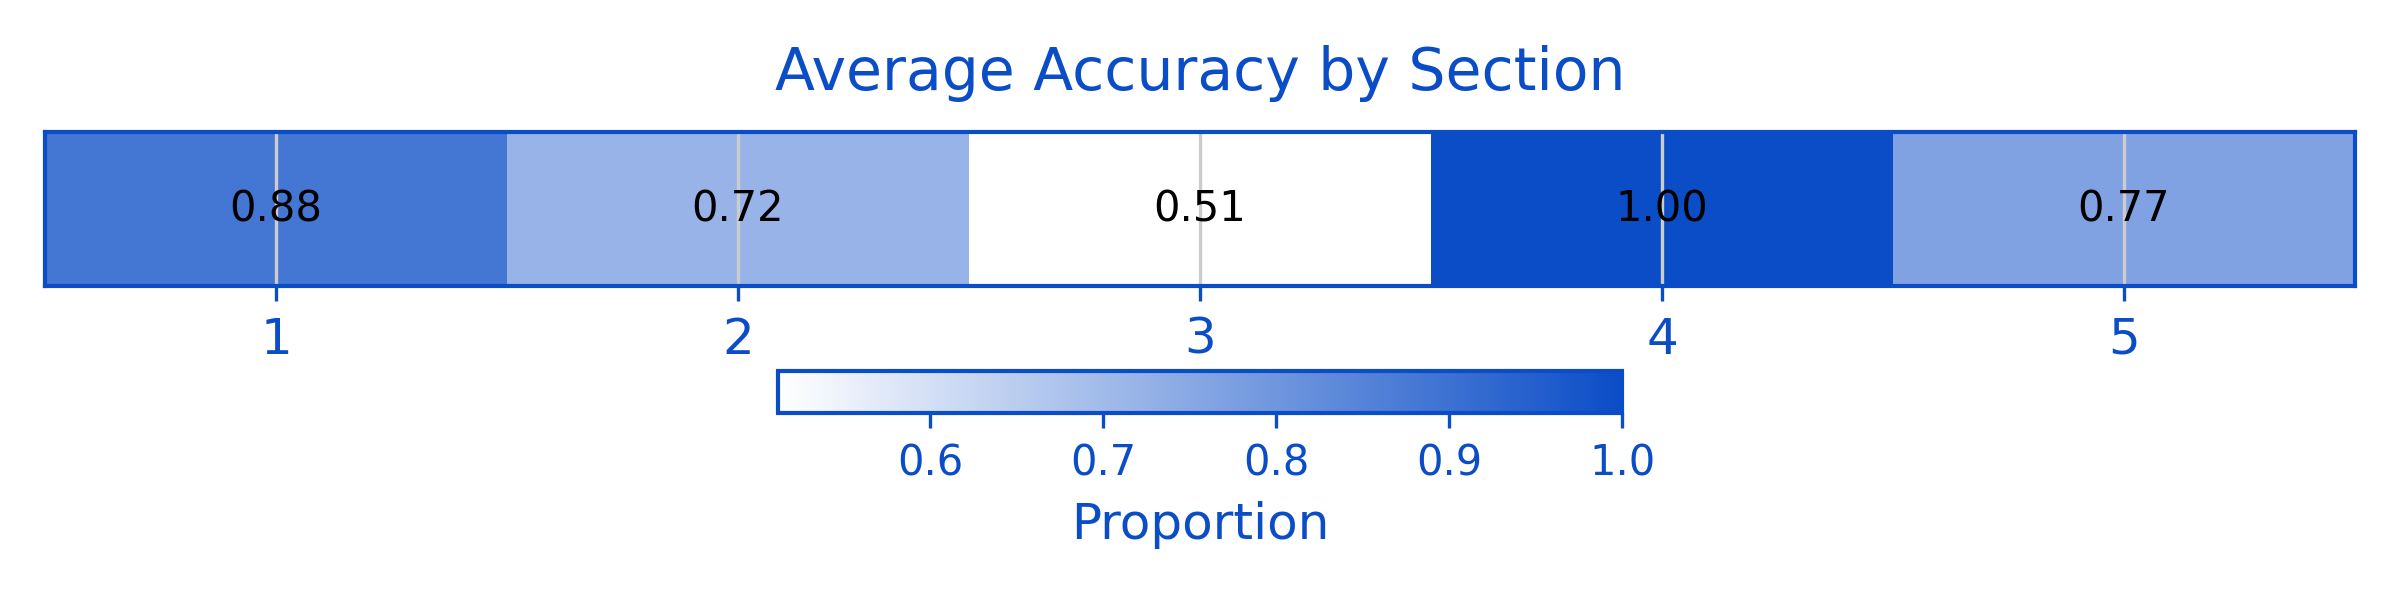
\includegraphics[width=0.8\textwidth]{figures/heatmap_accuracy.png}
\caption{Average Correctness Accuracy per task}
\label{fig:acc_hm}
{\raggedright \small{Source: created by the author based on project data}\par}
\end{figure}

The final heatmap from Figure \ref{fig:q_hm} shows the average time spent per question in each task. 
Task 3 clearly required more thinking with an average of 7.6 seconds but again did not lead to much improved results. 
Tasks 2 and 5 are roughly similar in time required for completion, which is a moderate challenge. 
Task 1 was twice as quick to complete per question in comparison, and with more questions, or rather cards to sort, serves more as a quick-fire intro to settle people in with the interactivity of the website.

\begin{figure}[hbtp]
\centering
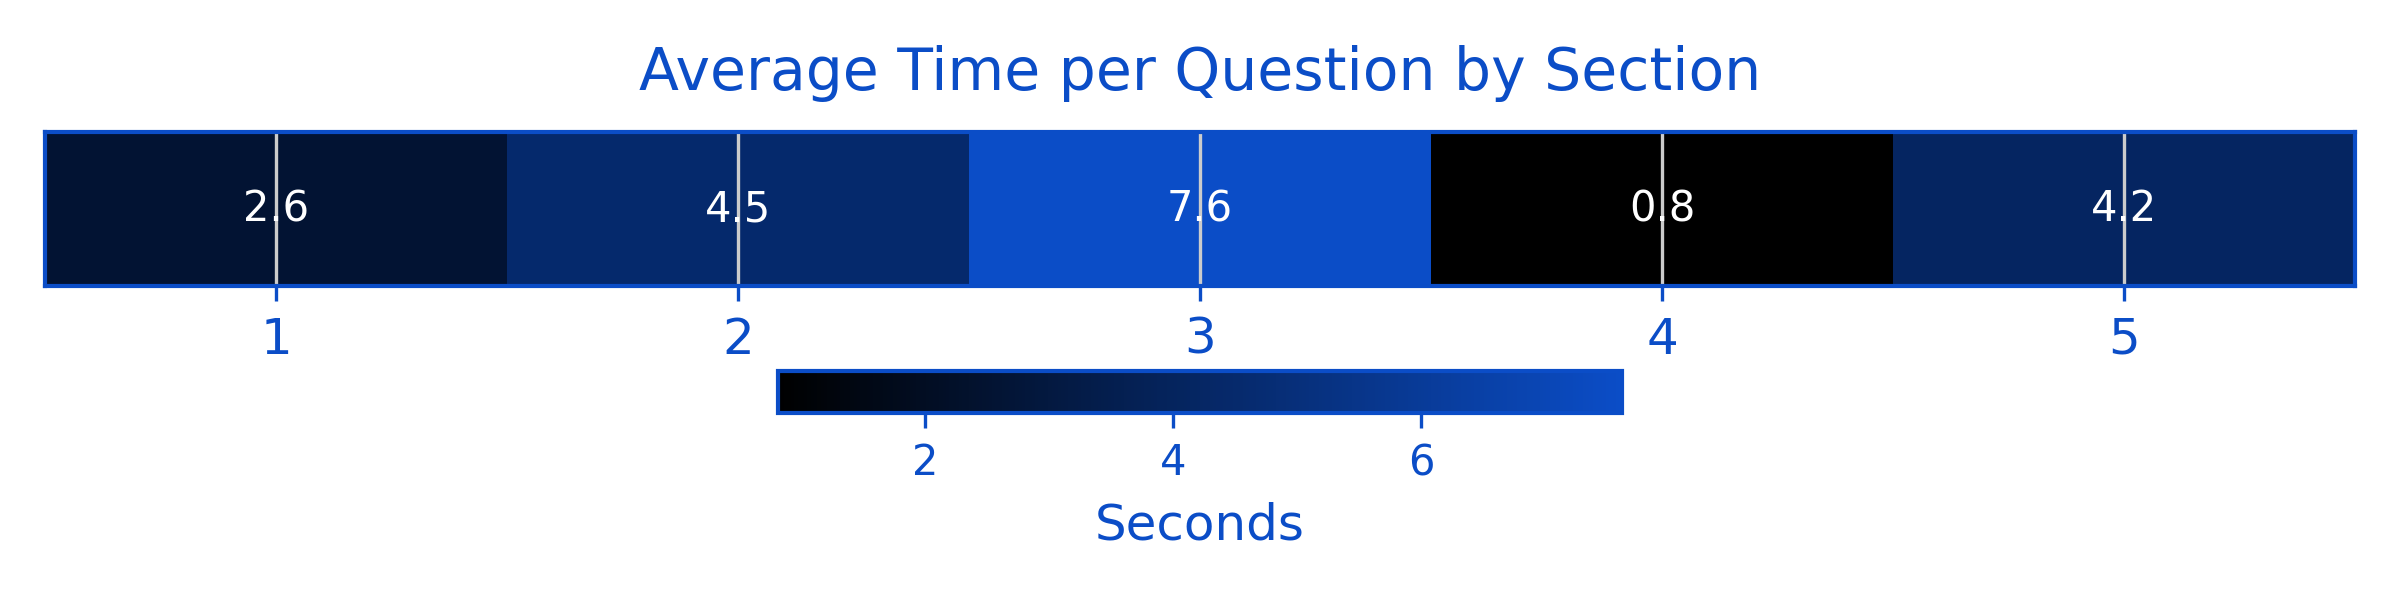
\includegraphics[width=0.8\textwidth]{figures/heatmap_time_per_q.png}
\caption{Average Time per Question by task}
\label{fig:q_hm}
{\raggedright \small{Source: created by the author based on project data}\par}
\end{figure}

\subsubsection{Survey Analysis}

The survey post-completion provided insights into user perception of gamification, enjoyment, and conceptual understanding. 
The numeric results of which can be seen within Table \ref{tab:survey_stats}. 
It has to be reiterated that the respondents were able to select answers between 1 and 4.
Overall sentiment was positive, but differences between categories and within questions revealed some minor insights:

\begin{itemize}
        \item Understanding received the highest ratings, with most users strongly agreeing they now understand Open Badges and their meaning, with mean scores of 3.78 and 3.56, respectively. 
        This confirms that the core educational objective was met successfully.
        \item Enjoyment scores were also consistently high, particularly for the overall website experience, with a mean of 3.67. 
        Navigation and interface satisfaction were likewise strong, with relatively low standard deviation, indicating consistent user satisfaction.
        \item Gamification results were mixed. The highest-rated statement was about interactive tasks enhancing engagement with a mean of 3.56. 
        The lowest result was from the question of whether the badge is a meaningful reward, which scored a mean of 2.89. 
        This disparity was statistically tested using a paired t-test, which returned a non-significant result p = 0.282, suggesting no strong divergence in user sentiment but rather mild skepticism toward the end reward's impact. 
        This is likely due to the certain stigma attached to all badges inherently, which the website is meant to reduce.
\end{itemize}

The correlation matrix further revealed a moderate positive association with a coefficient of 0.47 between Gamification and Enjoyment, indicating that users who felt engaged by the gamified elements also tended to enjoy the platform overall. However, this was not strong enough to claim a causal link.

Internal consistency analysis using Cronbach’s alpha returned:

0.71 for Gamification — acceptable and suggesting a coherent perception among the related items,

0.61 for Enjoyment — borderline, but interpretable, especially with the small sample size.

\begin{table}[ht]
{\small
\centering
\captionsetup{justification=raggedright, singlelinecheck=false}
\caption{Descriptive statistics of survey results}
\label{tab:survey_stats}
\begin{tabular}{|p{4.5cm}|c|c|c|c|c|}
\hline
\textbf{Statement} & \textbf{Category} & \textbf{Mean} & \textbf{SD} & \textbf{Min--Max} & \textbf{r with Enjoyment} \\
\hline
The interactive tasks made the learning experience more engaging. & Gamification & 3.56 & 0.53 & 3--4 & -0.16 \\
\hline
The score system engaged me to learn more. & Gamification & 3.22 & 0.83 & 2--4 & 0.20 \\
\hline
Receiving a badge at the end felt like a meaningful reward. & Gamification & 2.89 & 0.78 & 2--4 & -0.11 \\
\hline
Was the website enjoyable to use overall? & Enjoyment & 3.67 & 0.50 & 3--4 & \textemdash \\
\hline
The website was easy to navigate and worked well on my device. & Enjoyment & 3.44 & 0.53 & 3--4 & 0.16 \\
\hline
I would recommend this site to someone interested in learning about Open Badges. & Enjoyment & 3.44 & 0.73 & 2--4 & 0.46 \\
\hline
I better understand the concept of Open Badges after completing this website. & Understanding & 3.78 & 0.44 & 3--4 & -0.38 \\
\hline
I understand what the issued badge represents and how it could be used. & Understanding & 3.56 & 0.73 & 2--4 & -0.11 \\
\hline
\end{tabular}
}
\end{table}
{\raggedright \small{Source: based on results from author's implementation}\par}

\subsubsection{Qualitative Feedback Themes}
\begin{itemize}
    \item The general sentiment was that Task 1 was the favourite, due to being "Simple but effective" and particularly clear.
    \item In terms of difficulty, Task 3 was mentioned as the least favourable task due to a lack of clarity, increased failure and therefore, unfair loss of points.
    \item Over 80\% of respondents claim that interactive elements did not confuse or distract from the learning experience, and exclusively improved it. Notably, a comment that did describe distraction states that the distraction is rather an incite for the user to learn more and be more attentive rather than confusing.
    \item No respondents stated that the point scoring system hindered the user, some users stated that it had no impact, and the majority stated that it helped their performance.
    \item Within the freeform comment section, a couple of comments were made regarding niche mobile displays having minor visual issues. 
    Additionally, a user stated that the metaphorical "magic" in each step of the website is much appreciated.
\end{itemize}

\subsection{Analysis Conclusions}

The evaluation demonstrates that the implemented educational website effectively achieved its primary objective: helping users understand the core concepts of Open Badges. 
Quantitative data confirms that most tasks were performed with reasonable accuracy, and the post-survey results show a high level of user satisfaction and self-reported learning.

Task-level analysis identified Task 3 as a pain point for users. 
It had the lowest accuracy and highest time of completion, signalling a need for restructuring. 
Conversely, Task 4 was completed consistently completed quickly and flawlessly, due to an entirely different approach of being a leisurely activity in the middle of the user's journey.
Task 1 was praised both qualitatively and quantitatively for its clarity and relevance.

The survey results indicate strong user enjoyment and solid perceived learning outcomes. 
While gamification features were generally well received, the final badge reward was met with some scepticism, possibly due to broader perceptions of badge value. 
The moderate correlation between enjoyment and gamification suggests that while game elements enhanced engagement, they were not the sole driver of satisfaction.

Written feedback supported these conclusions, highlighting both the clarity of earlier tasks and the difficulty of more abstract ones. 
The progression system and interactivity were well received, with no critical usability issues apart from minor display bugs on specific devices.

Despite technical issues that reduced the sample size, the evaluation offers actionable insights: refine vague or overly punishing tasks, increase the reward perception of badges, and preserve what users already find intuitive and engaging. 

\subsection{Limitations and Suggestions for Future Research}

While this evaluation yielded valuable insights, several limitations must be acknowledged that may have affected the generalizability and depth of the findings.

\textbf{1. Small and Partially Corrupted Dataset.}
Due to technical issues with the backend infrastructure, several participant records were either lost or incomplete. 
This significantly reduced statistical power and increased the potential for bias or outlier influence. 
Future research should ensure more robust data integrity mechanisms and aim for a larger, more diverse sample.

\textbf{2. Limited Demographic and Contextual Data.}
No demographic data (e.g., age, digital literacy, or educational background) was collected. 
Such a decision was made due to the small sample size and a biased audience during promotion. 
Primarily, students between the ages of 20 to 30 participated in the data collection. 
As such, it is difficult to assess how prior knowledge or user context influenced learning outcomes or engagement. 
Future studies may benefit from anonymous profiling to better understand how different user types interact with the system.

\textbf{3. Subjective Survey Bias.}
The use of a 4-point Likert scale without a neutral midpoint was intentional to avoid indecision but may have pressured some users into selecting positions that did not fully represent their views. 
Additionally, social desirability bias may have influenced positively skewed responses, especially in small group settings. 
With a larger data sample, the Likert scale could be expanded for greater deviation

\textbf{4. Ambiguity in Task Design.}
The evaluation revealed that Task 3, while well-intentioned, resulted in substantial confusion and disproportionately low scores despite higher effort. 
Future research could be conducted with pilot testing and more rigorous usability reviews of task instructions and mechanics during the design phase.

\textbf{5. Badge Perception Uncertainty.}
Though central to the site's concept, the issued badge was not perceived as strongly meaningful by all users. 
This reflects a broader challenge with Open Badge literacy and acceptance. 
Future work should explore how contextual framing, real-world examples, or even credential-linked integration can enhance the perceived value of the badge system. 

\subsubsection{Recommendations for Future Research:}
\begin{itemize}
\item Recruit a larger and more varied user base to validate performance and perception trends across demographics.
\item Include pre-testing to track changes in user perception of Open Badges and their learning recognition.
\item Experiment with different reward systems or badge types to evaluate what design patterns better convey meaningfulness.
\item Introduce A/B testing for different task versions, e.g., with vs. without feedback or timed vs. untimed, to identify the most effective instructional strategies.
\item Consider longitudinal studies to explore how badge understanding or motivation changes over time.
\item Introduce additional requirements or reward tiers that have to be reached through excellent performance, to obtain the badge, as it is currently given as a participation trophy: everyone is capable of finishing the website regardless of the number of mistakes.
\end{itemize}

By addressing these limitations, future research can build a more complete and nuanced understanding of how gamified learning environments—and Open Badge systems specifically—can best support digital skill recognition and learner engagement.

\newpage
\newpage
\section*{CONCLUSIONS}
\addcontentsline{toc}{section}{CONCLUSIONS}
\begin{enumerate}
    \item \textbf{Theoretical Foundations} The analysis of gamification and open badge theory provided a strong foundation for the platform’s design. 
    The implementation successfully applied key motivational principles of \acrshort{sdt}, flow theory and \acrshort{mda}, leading to high user engagement and positive feedback in both structured tasks and open-ended responses. 
    This theoretical grounding was essential in ensuring that gamification elements like score feedback, progression, and reward systems were meaningful and not superficial.
    \item \textbf{Requirements and Design Specification} The functional and technical requirements identified early in the process, such as a mobile-first layout, structured task progression, and minimal cognitive friction, proved effective. 
    The feedback and performance data indicate that the site's architecture, section flow, and interaction model met usability and accessibility expectations, particularly for the intended higher education student audience.
    \item \textbf{Platform Development} The developed prototype successfully incorporated interactive, gamified elements that educated users about Open Badges. 
    The sequential task design consistently improved badge literacy in a clear and engaging way, with small, gamified tasks of card sorting, item selection and card association showing good learning impact. 
    The scenario identification task revealed issues with clarity. 
    The overall structure demonstrated that gamification could support and even enhance educational messaging when implemented thoughtfully.
    \item \textbf{Testing and Evaluation} The evaluation confirmed that the platform achieved its learning goals, with strong self-reported user understanding and enjoyment. 
    The mixed performance results and feedback highlighted specific areas for refinement, most notably the clarity and structure of task 3 and badge value perception. 
    Despite technical setbacks and a limited sample size, the testing methodology yielded actionable insights, validating both the concept and its execution while identifying concrete paths for improvement in future iterations and research.
\end{enumerate}

\newpage
% ------------------------------------------------------------------- SKYRIUS --
% ------------------------------------------------------------------- IŠVADOS --
%\section*{CONCLUSIONS}
%\phantomsection
%\addcontentsline{toc}{section}{CONCLUSIONS}
%
\phantomsection
\addcontentsline{toc}{section}{REFERENCES}
\printbibliography[title=REFERENCES]
\newpage
\appendix

\phantomsection
\begin{center}
    \Large \textbf{APPENDICES}
\end{center}
\vspace{1cm}

\appendixtitle{Appendix 1. User Survey Questionnaire}{Appendix 1. \textnormal{User Survey Questionnaire}}
\label{appendix:survey}
\vspace{0.5em}

The following appendix contains the complete list of user survey questions used in the study.

Questions were made available in both English and Lithuanian. Rated questions were within a scale of 1-4, with 1 as "Strongly disagree" and 4 as "Strongly agree".
\begin{enumerate}
  \item Choose your preferred language. Choice between English and Lithuanian.

  \textbf{Content and Clarity}
  \item I better understand the concept of Open Badges after completing this website. Rated 1-4.
  \item I understand what the issued badge represents and how it could be used. Rated 1-4.
  \item Which task or activity did you find the most useful or engaging for understanding Open Badges? Why? Open question.
  \item Which task or activity was the least helpful or enjoyable? Why? Open question.
  
  \textbf{Gamification and User Interaction}
  \item The interactive tasks made the learning experience more engaging. Rated 1-4.
  \item Did the interactive elements ever confuse or distract you from the learning content? Yes or No question.
  \item If you answered "Yes" in the previous question, please describe what confused or distracted you, and why. Open question.
  \item Did the progression system (unlocking sections as you go) help or hinder your learning experience? Rated from “Hindered” to “Helped”, with a “Not sure” and “Had no effect” as extra options.
  \item The score system engaged me to learn more. Rated 1-4.
  \item Receiving a badge at the end felt like a meaningful reward. Rated 1-4.

  \textbf{Usability and General Experience}
  \item The website is enjoyable to use overall. Rated 1-4.
  \item The website was easy to navigate and worked well on my device. Rated 1-4.
  \item I would recommend this site to someone interested in learning about Open Badges. Rated 1-4.
  \item Any other comments, suggestions, or technical issues you encountered? Open question.
\end{enumerate}

\newpage
\appendixtitle{Appendix 2. External Resources}{Appendix 2. \textnormal{External Resources}}
\label{appendix:external_resources}

The following appendix contains the complete list of links related to the project and its transparency.

\vspace{0.5em}
\begin{itemize}
  \item Prototype website link: \url{https://atvirieji-zenkliukai.netlify.app/}
  \item Backend API endpoint: \url{https://frontend-openbadges-bachelor.onrender.com/}
  \item Backend list of user sessions: \url{https://frontend-openbadges-bachelor.onrender.com/api/sessions}
  \item Individual user session results. Please replace "sessionId" with any session ID from the previous link: \url{https://frontend-openbadges-bachelor.onrender.com/api/logs/sessionId}
  \item Full source code: \url{https://github.com/MindaugasKazlavickas/Frontend_OpenBadges_Bachelor}
  \item This LaTeX thesis: \url{https://github.com/MindaugasKazlavickas/Thesis_OpenBadges_Bachelor}
\end{itemize}

\textit{Note: The hosted websites on Netlify and Render are intended to be maintained and freely available online until at least June 2026.}
\textit{Note: Badge issuance tied to Open Badge Factory is a paid service and will only be supported until mid-June of 2025. Afterwards attempted badge requests will result a "Something went wrong" error 500.}
\end{document}
% ------------------------------------------------------------------------------
%  DOKUMENTO PABAIGA
% ------------------------------------------------------------------------------
